% !TEX program = xelatex
% ZenOffice User Manual — shared Chinese / English content
% Representative UI screenshots were captured from an earlier release; this guide is updated for v0.6.72.
\documentclass[11pt,a4paper]{article}

% Edition wrappers define exactly one of these switches before inputting this file.
% With neither switch defined, the original bilingual combined edition is produced.
\newif\ifManualChineseOnly
\newif\ifManualEnglishOnly
\ifdefined\ZenOfficeChineseEdition
  \ManualChineseOnlytrue
\else\ifdefined\ZenOfficeEnglishEdition
  \ManualEnglishOnlytrue
\fi\fi

\ifManualChineseOnly
  \newcommand{\CNText}[1]{#1}
  \newcommand{\ENText}[1]{}
  \newcommand{\ManualEditionLine}{中文版 · Chinese Edition}
  \newcommand{\ManualFooter}{ZenOffice 快速入门指南 · 中文版}
  \newcommand{\ManualPdfTitle}{ZenOffice 快速入门指南（中文版）}
  \newcommand{\ManualPdfSubject}{ZenOffice v0.6.72 中文用户指南}
\else\ifManualEnglishOnly
  \newcommand{\CNText}[1]{}
  \newcommand{\ENText}[1]{#1}
  \newcommand{\ManualEditionLine}{English Edition · 英文版}
  \newcommand{\ManualFooter}{ZenOffice User Manual · English Edition}
  \newcommand{\ManualPdfTitle}{ZenOffice User Manual (English Edition)}
  \newcommand{\ManualPdfSubject}{ZenOffice v0.6.72 English user manual}
\else
  \newcommand{\CNText}[1]{#1}
  \newcommand{\ENText}[1]{#1}
  \newcommand{\ManualEditionLine}{中英双语合订本 · Chinese--English Bilingual Edition}
  \newcommand{\ManualFooter}{中英双语入门手册 · Bilingual Getting-Started Manual}
  \newcommand{\ManualPdfTitle}{ZenOffice 用户入门手册 / User Manual}
  \newcommand{\ManualPdfSubject}{ZenOffice v0.6.72 bilingual getting-started manual}
\fi\fi

\usepackage[a4paper,top=19mm,bottom=18mm,left=18mm,right=18mm,headheight=22pt]{geometry}
\usepackage{fontspec}
\usepackage{xeCJK}
\usepackage{amsmath,amssymb}
\usepackage{graphicx}
\usepackage{xcolor}
\usepackage{tikz}
\usetikzlibrary{positioning}
\usepackage{tabularx}
\usepackage{booktabs}
\usepackage{array}
\usepackage{enumitem}
\usepackage{fancyhdr}
\usepackage{hyperref}
\usepackage{bookmark}
\usepackage{microtype}
\usepackage{ragged2e}
\usepackage{setspace}
\usepackage{titlesec}

\defaultfontfeatures{Ligatures=TeX}
\setmainfont{Avenir Next}
\setsansfont{Avenir Next}
\setmonofont{Menlo}[Scale=0.82]
\setCJKmainfont{Hiragino Sans GB}
\setCJKsansfont{Hiragino Sans GB}
\setCJKmonofont{Hiragino Sans GB}
\newfontfamily\displayfont{Athelas}
\newCJKfontfamily\cjkdisplay{Hiragino Sans GB}

\definecolor{GOPaper}{HTML}{F1EFE7}
\definecolor{GOInk}{HTML}{161714}
\definecolor{GOMuted}{HTML}{66685F}
\definecolor{GOLine}{HTML}{C9C7BC}
\definecolor{GOBlue}{HTML}{2357FF}
\definecolor{GOAcid}{HTML}{D8FF42}
\definecolor{GORed}{HTML}{D83A2E}
\definecolor{GOWord}{HTML}{3478D4}
\definecolor{GOSheet}{HTML}{4DA36B}
\definecolor{GOSlide}{HTML}{DE3C25}
\definecolor{GOMarkdown}{HTML}{8754E9}
\definecolor{GOPdf}{HTML}{EF4056}
\definecolor{GOLight}{HTML}{F7F7F4}

\pagecolor{GOPaper}
\color{GOInk}
\graphicspath{{assets/screenshots/}}
\hypersetup{
  unicode=true,
  colorlinks=true,
  linkcolor=GOBlue,
  urlcolor=GOBlue,
  citecolor=GOBlue,
  pdftitle={\ManualPdfTitle},
  pdfauthor={ZenOffice contributors; AI adaptation by Zhiping Xu},
  pdfsubject={\ManualPdfSubject},
  pdfkeywords={ZenOffice, ZenMux, Word, Excel, PowerPoint, Markdown, PDF, AI}
}

\pagestyle{fancy}
\fancyhf{}
\fancyhead[L]{\footnotesize\bfseries ZenOffice \textcolor{GOBlue}{/} ZenMux}
\fancyhead[R]{\footnotesize\color{GOMuted} v0.6.72 · 2026-09-01}
\fancyfoot[L]{\scriptsize\color{GOMuted}\ManualFooter}
\fancyfoot[R]{\colorbox{GOBlue}{\makebox[8mm][c]{\color{white}\bfseries\thepage}}}
\renewcommand{\headrulewidth}{0.4pt}
\renewcommand{\headrule}{\hbox to\headwidth{\color{GOLine}\leaders\hrule height \headrulewidth\hfill}}

\setlength{\parindent}{0pt}
\setlength{\parskip}{5pt}
\setlength{\emergencystretch}{2em}
\setlist[itemize]{leftmargin=5.5mm,itemsep=3.5pt,topsep=4pt,label=\textcolor{GOBlue}{\small$\blacksquare$}}
\setlist[enumerate]{leftmargin=7mm,itemsep=4pt,topsep=4pt,label=\textcolor{GOBlue}{\bfseries\arabic*.}}
\setcounter{tocdepth}{2}
\ifManualChineseOnly
  \renewcommand{\contentsname}{目录}
\else\ifManualEnglishOnly
  \renewcommand{\contentsname}{Contents}
\else
  \renewcommand{\contentsname}{目录 · Contents}
\fi\fi
\titleformat{\section}{\Large\bfseries}{}{0pt}{}

\newcommand{\Kicker}[2]{%
  \noindent\colorbox{GOAcid}{\strut\hspace{2mm}\footnotesize\bfseries #1\hspace{2mm}}%
  \hfill{\footnotesize\color{GOMuted}#2}\par\vspace{5mm}}

\newcommand{\TopicTitle}[2]{%
  {\raggedright\cjkdisplay\displayfont\fontsize{28}{32}\selectfont\bfseries #1\par}%
  \vspace{1.5mm}
  {\raggedright\displayfont\fontsize{16}{19}\selectfont\color{GOBlue}#2\par}%
  \vspace{4mm}}

\newcommand{\Lead}[1]{%
  \begin{tikzpicture}
    \node[fill=white,draw=GOLine,rounded corners=2pt,inner sep=4mm,text width=.925\linewidth,align=left]
      {\large\color{GOInk}#1};
  \end{tikzpicture}\par\vspace{3mm}}

\newcommand{\Tip}[2][提示 · Tip]{%
  \vspace{2mm}
  \begin{tikzpicture}
    \node[fill=GOAcid!45,draw=GOInk,rounded corners=2pt,inner sep=3.5mm,text width=.93\linewidth,align=left]
      {\footnotesize\bfseries #1\quad\normalfont #2};
  \end{tikzpicture}}

\newcommand{\Warn}[1]{%
  \vspace{2mm}
  \begin{tikzpicture}
    \node[fill=GORed!7,draw=GORed,rounded corners=2pt,inner sep=3.5mm,text width=.93\linewidth,align=left]
      {\footnotesize\color{GORed}\bfseries 注意 · Notice\quad\normalfont\color{GOInk}#1};
  \end{tikzpicture}}

\newcommand{\Shot}[2]{%
  \vspace{2mm}
  \begin{center}
    \fcolorbox{GOLine}{white}{\includegraphics[width=.91\linewidth]{#1}}\\[-1mm]
    {\scriptsize\color{GOMuted}#2}
  \end{center}}

\newcommand{\SmallShot}[2]{%
  \begin{center}
    \fcolorbox{GOLine}{white}{\includegraphics[width=.76\linewidth]{#1}}\\[-1mm]
    {\scriptsize\color{GOMuted}#2}
  \end{center}}

\newcommand{\AppStrip}{%
  \begin{center}\begin{tikzpicture}[x=1cm,y=1cm]
    \foreach \x/\c/\t in {0/GOWord/W,1.55/GOSheet/X,3.1/GOSlide/P,4.65/GOMarkdown/MD,6.2/GOPdf/PDF} {
      \node[fill=\c,text=white,rounded corners=3pt,minimum width=1.25cm,minimum height=1.1cm,font=\bfseries] at (\x,0) {\t};
    }
    \draw[GOBlue,very thick,-stealth] (6.95,0) -- (8.4,0);
    \node[fill=GOInk,text=white,rounded corners=3pt,minimum width=1.55cm,minimum height=1.1cm,font=\bfseries] at (9.3,0) {ZenMux};
  \end{tikzpicture}\end{center}}

\newcommand{\Flow}[4]{%
  \begin{center}\begin{tikzpicture}[node distance=7mm]
    \node[draw=GOLine,fill=white,rounded corners=2pt,text width=31mm,minimum height=13mm,align=center] (a) {\small\bfseries #1};
    \node[draw=GOLine,fill=white,rounded corners=2pt,text width=31mm,minimum height=13mm,align=center,right=of a] (b) {\small\bfseries #2};
    \node[draw=GOLine,fill=white,rounded corners=2pt,text width=31mm,minimum height=13mm,align=center,right=of b] (c) {\small\bfseries #3};
    \node[draw=GOBlue,fill=GOBlue,text=white,rounded corners=2pt,text width=31mm,minimum height=13mm,align=center,right=of c] (d) {\small\bfseries #4};
    \draw[-stealth,thick,GOBlue] (a)--(b);
    \draw[-stealth,thick,GOBlue] (b)--(c);
    \draw[-stealth,thick,GOBlue] (c)--(d);
  \end{tikzpicture}\end{center}}

\ifManualEnglishOnly
\newcommand{\CNPage}[5]{}
\else
\newcommand{\CNPage}[5]{%
  \clearpage\phantomsection
  \ifManualChineseOnly
    \addcontentsline{toc}{subsection}{#1\space #2}
  \else
    \addcontentsline{toc}{subsection}{#1\space #2 / #3}
  \fi
  \pdfbookmark[2]{#2 / #3}{topic-#1-cn}
  \Kicker{#1 · 中文}{ZENOFFICE FIELD GUIDE}
  \TopicTitle{#2}{#3}
  \Lead{#4}
  #5
}
\fi

\ifManualChineseOnly
\newcommand{\ENPage}[5]{}
\else
\newcommand{\ENPage}[5]{%
  \clearpage\phantomsection
  \ifManualEnglishOnly
    \addcontentsline{toc}{subsection}{#1\space #3}
  \fi
  \pdfbookmark[2]{#3 / #2}{topic-#1-en}
  \Kicker{#1 · ENGLISH}{ZENOFFICE FIELD GUIDE}
  \TopicTitle{#3}{#2}
  \Lead{#4}
  #5
}
\fi

\newcommand{\PartPage}[5]{%
  \clearpage\phantomsection
  \ifManualChineseOnly
    \addcontentsline{toc}{section}{#1\space #2}
  \else\ifManualEnglishOnly
    \addcontentsline{toc}{section}{#1\space #3}
  \else
    \addcontentsline{toc}{section}{#1\space #2 / #3}
  \fi\fi
  \pdfbookmark[1]{#2 / #3}{part-#1}
  \thispagestyle{empty}
  \begin{tikzpicture}[remember picture,overlay]
    \fill[GOBlue] (current page.south west) rectangle (current page.north east);
    \fill[GOAcid] ([xshift=18mm,yshift=-20mm]current page.north west) rectangle ++(33mm,-7mm);
    \draw[white!35,line width=.6pt] ([xshift=18mm,yshift=-35mm]current page.north west) -- ([xshift=-18mm,yshift=-35mm]current page.north east);
  \end{tikzpicture}
  \vspace*{32mm}
  {\color{white}\fontsize{18}{21}\selectfont\bfseries PART #1\par}
  \vspace{25mm}
  \CNText{{\color{white}\cjkdisplay\displayfont\fontsize{39}{46}\selectfont\bfseries #2\par}}
  \ifManualChineseOnly\else\vspace{3mm}\fi
  \ENText{{\color{GOAcid}\displayfont\fontsize{24}{29}\selectfont\itshape #3\par}}
  \vfill
  \CNText{{\color{white!80}\large #4\par}}
  \ENText{{\color{white!80}\large #5\par}}
  \vspace{18mm}
}

\begin{document}

% -----------------------------------------------------------------------------
% Cover
% -----------------------------------------------------------------------------
\thispagestyle{empty}
\begin{tikzpicture}[remember picture,overlay]
  \fill[GOInk] (current page.south west) rectangle (current page.north east);
  \fill[GOBlue] ([xshift=24mm,yshift=-24mm]current page.north west) rectangle ++(45mm,-10mm);
  \fill[GOAcid] ([xshift=-62mm,yshift=24mm]current page.south east) rectangle ++(38mm,10mm);
  \draw[white!18,line width=.6pt] ([xshift=24mm,yshift=-46mm]current page.north west) -- ([xshift=-24mm,yshift=-46mm]current page.north east);
  \draw[white!18,line width=.6pt] ([xshift=24mm,yshift=48mm]current page.south west) -- ([xshift=-24mm,yshift=48mm]current page.south east);
\end{tikzpicture}
\vspace*{18mm}
{\color{white}\bfseries\large Z/O \hspace{3mm} ZenOffice}\par
\vspace{38mm}
\CNText{{\color{white}\cjkdisplay\fontsize{41}{48}\selectfont\bfseries 快速入门指南\par}}
\ifManualChineseOnly\else\vspace{4mm}\fi
\ENText{{\color{GOAcid}\displayfont\fontsize{28}{34}\selectfont\itshape User Manual\par}}
\vspace{12mm}
\CNText{{\color{white!76}\Large ZenMux 驱动的本地 AI 办公工作台\par}}
\ENText{{\color{white!76}\Large ZenMux-powered local AI office workspace\par}}
\vfill
\AppStrip
\vfill
{\color{white}\bfseries\ManualEditionLine\par}
{\color{white!70}\small v0.6.72 · 2026-09-01 · macOS / Windows / Ubuntu / RPM\par}
\clearpage

% -----------------------------------------------------------------------------
% Credits and provenance
% -----------------------------------------------------------------------------
\thispagestyle{empty}
\Kicker{版本与版权 · Edition \& Credits}{SOURCE-VERIFIED MANUAL}
\TopicTitle{关于本手册}{About this manual}

\CNText{本手册面向第一次使用 ZenOffice 的用户，以当前仓库 \textbf{v0.6.72} 源码与真实运行态为依据，说明安装、ZenMux 设置、Word、Excel、PowerPoint、Markdown、PDF、工作簿 SQL 数据库、跨平台打印以及跨编辑器 AI 工作流。界面截图于 2026-08-16 至 17 日在隔离的临时用户目录中从应用运行态取得；截图没有包含用户文件、真实 API Key 或个人数据。演示科研稿与工作簿均为专门制作的合成素材，不代表真实科研或企业结论。}

\ENText{This manual is based on the current \textbf{v0.6.72} source tree and real runtime UI. It covers installation, ZenMux configuration, Word, Excel, PowerPoint, Markdown, PDF, workbook SQL databases, cross-platform printing, and cross-editor AI workflows. Screenshots were captured on 16--17 August 2026 in an isolated temporary profile and contain no user documents, real API Key, or personal data. The research draft and workbooks are purpose-built synthetic demonstrations, not real scientific or business findings.}

\vspace{5mm}
\begin{tikzpicture}
  \node[fill=white,draw=GOLine,rounded corners=2pt,inner sep=5mm,text width=.91\linewidth,align=left] {
    \textbf{AI 适配与修改 / AI adaptation and modifications}\\[2mm]
    \CNText{由复旦大学计算与智能创新学院徐志平完成 AI 适配与修改工作。}
    \ENText{AI adaptation and modifications by Zhiping Xu, College of Computer Science and Artificial Intelligence, Fudan University.}
  };
\end{tikzpicture}

\vspace{5mm}
\CNText{ZenOffice 是 \href{https://github.com/genspark-ai/genoffice}{genspark-ai/genoffice} 的衍生版本，保留 Apache-2.0 开源基础，并完成 ZenMux AI 通道、本地凭据、学术工作流、跨编辑器连接及多平台发行等适配。项目源码与发行包见 \href{https://github.com/bennix/GenZenMuxAIOffice}{bennix/GenZenMuxAIOffice}。}

\ENText{ZenOffice is derived from \href{https://github.com/genspark-ai/genoffice}{genspark-ai/genoffice}. It retains the Apache-2.0 foundation and adds ZenMux routing, local credential storage, academic workflows, cross-editor connections, and multi-platform distribution. Source and releases are available at \href{https://github.com/bennix/GenZenMuxAIOffice}{bennix/GenZenMuxAIOffice}.}

\Warn{AI 功能依赖网络、代理状态和模型服务可用性。AI 输出、联网结果、公式识别、审稿意见与图像生成均应由用户核对。AI features depend on network, proxy, and provider availability; always verify generated content, sources, formulas, reviews, and images.}

\vfill
{\small\color{GOMuted}\CNText{手册 LaTeX 源文件与生成的 PDF 同步发布。文档中的产品名称、第三方项目及商标归各自权利人所有。}\ENText{The LaTeX source and compiled PDF are published together. Product names, third-party projects, and trademarks belong to their respective owners.}}
\clearpage

% -----------------------------------------------------------------------------
% Reading map
% -----------------------------------------------------------------------------
\ifManualChineseOnly
  \Kicker{阅读地图}{从这里开始}
  \TopicTitle{一分钟找到需要的章节}{按任务直接跳转，不必从头阅读}
  \Lead{这是一份连续阅读的中文版。先完成 ZenMux 配置，再用“3 分钟尝鲜指南”跑通一个真实场景；其余章节可按 Word、Excel、PPT、Markdown 或 PDF 直接跳转。}
  \begin{tabularx}{\linewidth}{>{\bfseries}p{31mm} X}
  \toprule
  想完成什么 & 从哪里开始\\\midrule
  立即体验 & 第 I 部分后：3 分钟尝鲜指南\\
  使用 AI & 第 II 部分：选区、附件、复制、@Connect\\
  处理文件 & 第 III--VI 部分：Word、Excel、PPT、Markdown、PDF\\
  做科研工作 & 公式、文献、引用、审稿、联网查证\\
  快速排障 & 第 VII 部分与“一分钟故障排查表”\\
  \bottomrule
  \end{tabularx}
\else\ifManualEnglishOnly
  \Kicker{READING MAP}{START ANYWHERE}
  \TopicTitle{Find the right section in one minute}{Jump straight to the job you need to finish}
  \Lead{This is the continuous English edition. Configure ZenMux, complete one three-minute recipe, then jump directly to Word, Excel, PowerPoint, Markdown, or PDF. Screenshots use the Chinese UI while paths name the matching controls.}
  \begin{tabularx}{\linewidth}{>{\bfseries}p{38mm} X}
  \toprule
  Goal & Start here\\\midrule
  Try it now & Three-minute quick wins after Part I\\
  Use AI & Part II: selections, attachments, copy, and @Connect\\
  Work with files & Parts III--VI: Word, Excel, PPT, Markdown, PDF\\
  Research workflow & Equations, literature, citations, review, web verification\\
  Fix a problem & Part VII and the one-minute troubleshooting table\\
  \bottomrule
  \end{tabularx}
\else
  \Kicker{阅读地图 · Reading map}{START ANYWHERE}
  \TopicTitle{一分钟找到需要的章节}{Find the right section in one minute}
  \Lead{合订本保留中英文相邻主题；需要连续阅读时，推荐下载独立中文版或英文版。 / The combined edition keeps adjacent Chinese and English topics; use a separate language edition for uninterrupted reading.}
  \begin{tabularx}{\linewidth}{>{\bfseries}p{28mm} X X}
  \toprule
  目标 · Goal & 中文入口 & English route\\\midrule
  立即体验 & 第 I 部分后：3 分钟尝鲜指南 & Three-minute recipes after Part I\\
  使用 AI & 第 II 部分：上下文、附件、复制、@Connect & Part II: context, attachments, copy, @Connect\\
  编辑文件 & 第 III--VI 部分：Word、Excel、PPT、Markdown、PDF & Parts III--VI: Word, Excel, PPT, Markdown, PDF\\
  快速排障 & 第 VII 部分与一分钟故障排查表 & Part VII and one-minute troubleshooting\\
  \bottomrule
  \end{tabularx}
\fi\fi

\vspace{7mm}
\AppStrip

\vspace{5mm}
\CNText{\begin{itemize}
  \item 路径中的“设置 > AI 模型”表示先打开设置，再选择“AI 模型”。
  \item macOS 的 \textbf{Command} 与 Windows/Linux 的 \textbf{Ctrl} 写作 \textbf{Cmd/Ctrl}。
  \item AI 工作流需要用户自己的 ZenMux API Key；纯本地编辑不需要 Key。
  \item PDF 以查看、页面处理、水印、安全与 AI 问答为主；当前功能区不提供文字、图片或公式编辑入口。
\end{itemize}}
\ENText{\begin{itemize}
  \item “Settings > AI models” means open Settings, then choose AI models.
  \item \textbf{Cmd/Ctrl} means Command on macOS and Ctrl on Windows/Linux.
  \item AI workflows require your ZenMux API Key; local-only editing does not.
  \item PDF focuses on viewing, pages, watermarks, security, and AI Q\&A; its current ribbon does not expose text, image, or equation editing.
\end{itemize}}

\Tip{\CNText{先配置 ZenMux，再任选一个三分钟场景完成第一次闭环。}\ENText{Configure ZenMux first, then complete any three-minute recipe for your first end-to-end result.}}
\clearpage

\tableofcontents
\clearpage

% =============================================================================
% PART I — Start and configure
% =============================================================================
\PartPage{I}{安装与设置}{Install \& configure}{从可信发行包开始，完成首次启动，并把 ZenMux API Key 安全地保存在本机。}{Start from a trusted build, complete first launch, and store the ZenMux API Key securely on this device.}

\CNPage{01}{安装并验证应用}{Install and verify}{ZenOffice 提供 macOS DMG、Windows x64 安装程序、Ubuntu DEB 与通用 RPM。请只从项目 Landing Page 或 GitHub Releases 下载。}{
\begin{enumerate}
  \item 在 \href{https://bennix.github.io/GenZenMuxAIOffice/}{官方 Landing Page} 选择操作系统；检查页面显示的当前版本与文件名一致。
  \item macOS：打开 DMG，将 ZenOffice 拖入“应用程序”。Apple Silicon 版本使用 Developer ID 签名；是否包含 Apple 公证票据以对应 Release 的验证说明为准。
  \item Windows：运行 x64 安装程序。当前安装包未做 Authenticode 签名，SmartScreen 可能显示“未知发布者”；请核对下载域名与 Release 文件。
  \item Ubuntu：执行 \texttt{sudo apt install ./zenoffice\_0.6.72\_amd64.deb}。Fedora/RHEL 系使用 \texttt{sudo dnf install ./zenoffice-0.6.72.x86\_64.rpm}。
\end{enumerate}
\begin{center}
\begin{tabularx}{.95\linewidth}{>{\bfseries}p{28mm}p{43mm}X}
\toprule
平台 & 文件 & 说明\\\midrule
macOS & .dmg & Apple Silicon，macOS 11+\\
Windows & .exe & Windows 10/11 x64\\
Ubuntu & .deb & Ubuntu 22.04/24.04 amd64\\
RPM & .rpm & Fedora/RHEL/Rocky/Alma/openSUSE x86\_64\\
\bottomrule
\end{tabularx}
\end{center}
\Tip{安装包版本、Landing Page 版本与下载链接应一致。若浏览器下载失败，进入 GitHub Releases 后手动选择同名资源。}
}

\ENPage{01}{安装并验证应用}{Install and verify}{ZenOffice ships as a macOS DMG, Windows x64 installer, Ubuntu DEB, and RPM. Download only from the project Landing Page or GitHub Releases.}{
\begin{enumerate}
  \item Open the \href{https://bennix.github.io/GenZenMuxAIOffice/}{official Landing Page}, choose your platform, and confirm that the displayed version matches the filename.
  \item macOS: open the DMG and drag ZenOffice to Applications. The Apple Silicon build is Developer ID signed; consult the matching Release verification notes for notarization-ticket status.
  \item Windows: run the x64 installer. The current build is not Authenticode-signed, so SmartScreen may report an unknown publisher; verify the domain and Release asset first.
  \item Ubuntu: run \texttt{sudo apt install ./zenoffice\_0.6.72\_amd64.deb}. Fedora/RHEL-family users can run \texttt{sudo dnf install ./zenoffice-0.6.72.x86\_64.rpm}.
\end{enumerate}
\begin{center}
\begin{tabularx}{.95\linewidth}{>{\bfseries}p{28mm}p{43mm}X}
\toprule
Platform & File & Requirement\\\midrule
macOS & .dmg & Apple Silicon, macOS 11+\\
Windows & .exe & Windows 10/11 x64\\
Ubuntu & .deb & Ubuntu 22.04/24.04 amd64\\
RPM & .rpm & Fedora/RHEL/Rocky/Alma/openSUSE x86\_64\\
\bottomrule
\end{tabularx}
\end{center}
\Tip{The installer version, Landing Page label, and download target should agree. If a direct link fails, open GitHub Releases and choose the matching asset manually.}
}

\CNPage{02}{首次启动与欢迎页}{First launch and welcome}{欢迎页直接连接 ZenMux：可以立即填写 API Key，也可以先跳过，在设置页稍后完成。纯本地文件编辑不要求登录。}{
\SmallShot{01-onboarding-zenmux.png}{当前源码真实运行态：ZenMux 首次启动欢迎页（未填写任何真实凭据）。}
\begin{enumerate}
  \item 没有 API Key 时，点击邀请链接 \url{https://zenmux.ai/invite/GBQMC5} 申请或注册。
  \item 把 Key 粘贴到输入框，选择默认文本模型，然后继续。Key 会在界面中以遮罩形式显示。
  \item 暂时只想编辑本地文件时，可选择“跳过”；Word、Excel、PPT、Markdown 和 PDF 的非 AI 功能仍可使用。
\end{enumerate}
\Warn{不要把 API Key 写入文档正文、截图、聊天附件或公开仓库。应用设置页是唯一推荐的录入位置。}
}

\ENPage{02}{首次启动与欢迎页}{First launch and welcome}{The welcome screen connects directly to ZenMux. Enter an API Key now or skip and configure it later in Settings. Local file editing does not require sign-in.}{
\SmallShot{01-onboarding-zenmux.png}{Real runtime UI from the current source: ZenMux welcome screen with no real credential entered.}
\begin{enumerate}
  \item If you do not have a key, use \url{https://zenmux.ai/invite/GBQMC5} to register or request one.
  \item Paste the key, choose the default text model, and continue. The value is masked in the interface.
  \item To work locally first, choose Skip. Non-AI features in Word, Excel, PowerPoint, Markdown, and PDF remain available.
\end{enumerate}
\Warn{Never place an API Key in document text, screenshots, chat attachments, or a public repository. Settings is the recommended entry point.}
}

\CNPage{03}{主页、项目与最近文件}{Home, projects, and recent files}{主页集中提供五类编辑器、打开本地文件、项目列表、收藏和最近文件。一个窗口可以用标签页并行处理多种格式。}{
\Shot{02-home-quick-start.png}{当前源码真实运行态：主页快速新建卡片、项目栏、最近文件筛选与设置入口。}
\begin{itemize}
  \item 点击 AI Docs、AI Sheets、AI Slides、AI Markdown 或 AI PDF 新建对应内容；“打开本地文件”用于选择已有文件。
  \item 也可以把 DOC/DOCX、XLS/XLSX/CSV、PPTX、PDF 或 MD 文件直接拖到任意模块窗口；桌面外壳会识别真实格式并自动交给对应编辑器打开。
  \item 左侧“项目”用于组织文件；“最近”和“收藏”可快速返回经常使用的内容。
  \item 右侧筛选条按文档、表格、演示、PDF 或 Markdown 缩小最近文件范围。
\end{itemize}
\Tip{拖放用于打开文件，不会把原文件复制进当前文档。同一个文件已经在标签页中打开时，优先切回现有标签，避免产生两个编辑会话。}
}

\ENPage{03}{主页、项目与最近文件}{Home, projects, and recent files}{The home screen brings together five editors, local-file opening, projects, favorites, and recents. Tabs let one window host several file types.}{
\Shot{02-home-quick-start.png}{Real runtime UI: quick-create cards, project navigation, recent-file filters, and Settings.}
\begin{itemize}
  \item Choose AI Docs, AI Sheets, AI Slides, AI Markdown, or AI PDF to create content; Open local file selects an existing file.
  \item You may also drop DOC/DOCX, XLS/XLSX/CSV, PPTX, PDF, or Markdown onto any module window. The desktop shell detects the actual format and routes it to the matching editor automatically.
  \item Projects organize work. Recent and Favorites provide quick return paths.
  \item The filter strip narrows recents to documents, spreadsheets, presentations, PDF, or Markdown.
\end{itemize}
\Tip{Dropping opens the file; it does not insert a copy into the current document. If a file is already open, switch to that tab instead of creating a second editing session.}
}

\CNPage{04}{快速配置 AI 算力与模型}{Get AI ready: key, model, and connection test}{所有 AI 通道使用统一的 OpenAI 兼容地址 \url{https://zenmux.ai/api/v1}。录入 API Key、选择模型并完成一次短测试，即可开箱使用。}{
\SmallShot{03-settings-zenmux.png}{当前源码真实运行态：设置 > AI 模型；API Key 为空且界面不暴露任何秘密。}
\begin{enumerate}
  \item 在主页左下角点击“设置”，选择“AI 模型”。
  \item 粘贴 ZenMux API Key。Base URL 已锁定为 \url{https://zenmux.ai/api/v1}，通常不需要修改。
  \item 选择一个文本模型和一个配图模型，关闭设置。新配置会供 Word、Excel、PPT、Markdown 和 PDF 共用。
  \item 发送一条不含隐私内容的短问题验证连接；若失败，先检查网络、代理、额度和模型可用性。
\end{enumerate}
\Tip{设置页会遮罩 Key；保存使用操作系统安全存储。更换 Key 时直接在同一位置覆盖即可。}
}

\ENPage{04}{快速配置 AI 算力与模型}{Get AI ready: key, model, and connection test}{Every AI path uses the OpenAI-compatible endpoint \url{https://zenmux.ai/api/v1}. Enter the key, choose a model, and run one short test to get started.}{
\SmallShot{03-settings-zenmux.png}{Real runtime UI: Settings > AI models, with an empty API Key field and no secret exposed.}
\begin{enumerate}
  \item Select Settings at the lower left of Home, then open AI models.
  \item Paste the ZenMux API Key. The Base URL is fixed to \url{https://zenmux.ai/api/v1} and normally needs no change.
  \item Choose one text model and one illustration model, then close Settings. Word, Excel, PowerPoint, Markdown, and PDF share the configuration.
  \item Send a short, non-sensitive test question. If it fails, check network, proxy, quota, and model availability.
\end{enumerate}
\Tip{The UI masks the key and saves it through operating-system secure storage. Enter a replacement in the same field to rotate credentials.}
}

\CNPage{05}{增加、选择与删除模型}{Add, select, and remove models}{设置页既可选择预置模型，也可按 ZenMux 的 provider/model-name 格式增加模型；文本模型和配图模型都支持删除。}{
\SmallShot{03-settings-zenmux.png}{模型区真实运行态：当前模型、增加模型名称、配图模型与删除按钮。}
\begin{itemize}
  \item 本版预置文本模型：\nolinkurl{anthropic/claude-sonnet-4.6}、\nolinkurl{z-ai/glm-5v-turbo}、\nolinkurl{openai/gpt-5.4}。
  \item 公式图片识别默认视觉模型：\nolinkurl{z-ai/glm-5v-turbo}。
  \item 配图默认可使用：\nolinkurl{openai/gpt-image-2}。
  \item 新增时输入 ZenMux 模型页给出的完整名称，不要省略提供商前缀。加入后从下拉列表设为当前模型。
  \item 删除只会移除本地模型列表，不会删除 ZenMux 平台上的模型或账户数据。至少保留一个可用文本模型。
\end{itemize}
\Tip{不同图像模型的请求格式可能不同；优先使用应用已适配的模型。新模型若报参数错误，可先切回预置模型验证。}
}

\ENPage{05}{增加、选择与删除模型}{Add, select, and remove models}{Settings offers built-in models and accepts additional names in ZenMux provider/model-name form. Text and illustration models can both be removed locally.}{
\SmallShot{03-settings-zenmux.png}{Real runtime model area: current model, add-model field, illustration model, and delete controls.}
\begin{itemize}
  \item Built-in text models in this release: \nolinkurl{anthropic/claude-sonnet-4.6}, \nolinkurl{z-ai/glm-5v-turbo}, and \nolinkurl{openai/gpt-5.4}.
  \item Formula image recognition model: \nolinkurl{z-ai/glm-5v-turbo}.
  \item Illustration model: \nolinkurl{openai/gpt-image-2}.
  \item Add the complete name shown by ZenMux, including the provider prefix, then select it from the current-model list.
  \item Delete removes only the local list entry; it does not delete a ZenMux model or account data. Keep at least one working text model.
\end{itemize}
\Tip{Image models may require different request formats. Prefer models already adapted by the app; if a new model rejects parameters, switch back to a built-in model to isolate the issue.}
}

\CNPage{06}{确认隐私保护、版本与网络状态}{Verify privacy, version, and connectivity}{API Key 在界面中加密遮罩，并由系统凭据服务安全保存；“设置 > 关于”可核对版本、适配署名和更新通道。}{
\SmallShot{04-settings-about.png}{设置 > 关于的真实运行态；截图采集于旧版界面，发行与手册版本以页眉标注的 v0.6.72 为准。}
\begin{itemize}
  \item macOS 使用系统安全存储/钥匙串能力；Windows 使用系统凭据加密机制。应用不会把 Key 写进安装包或手册。
  \item 文档打开、编辑和保存以本地为主；调用 ZenMux、联网搜索、文献检索、公式 OCR 或配图时才需要网络。
  \item 网络、代理、服务负载、额度或某个模型的临时状态都可能影响速度和结果；超时不等于供应方一定没有生成结果。
  \item “关于”页用于核对实际安装版本。报告问题时附上版本、平台、操作路径和无敏感信息的截图。
\end{itemize}
\Warn{若怀疑 Key 泄露，应立即在 ZenMux 平台撤销或轮换，并在设置中替换；不要把 Key 发给支持人员。}
}

\ENPage{06}{确认隐私保护、版本与网络状态}{Verify privacy, version, and connectivity}{The API Key is masked and protected by the operating-system credential service. Settings > About confirms version, adaptation credit, and update channel.}{
\SmallShot{04-settings-about.png}{Real Settings > About runtime; the capture predates this release, so use the v0.6.72 header as the authoritative manual version.}
\begin{itemize}
  \item macOS uses operating-system secure storage/Keychain capabilities; Windows uses system credential encryption. The key is not embedded in installers or this manual.
  \item Opening, editing, and saving files are local-first. ZenMux calls, web search, literature search, formula OCR, and image generation require a network.
  \item Network, proxy, provider load, quota, or model status can affect speed and output. A client timeout does not prove that the provider produced no result.
  \item Use About to confirm the installed version. A useful issue report includes version, platform, action path, and a screenshot without secrets.
\end{itemize}
\Warn{If a key may be exposed, revoke or rotate it at ZenMux and replace it in Settings. Never send the key to support staff.}
}

% =============================================================================
% THREE-MINUTE COOKBOOK
% =============================================================================
\PartPage{I+}{3 分钟尝鲜指南}{Three-minute quick wins}{不先学习所有概念：任选一个真实场景，在三分钟内看见可编辑结果。}{Skip the theory at first: choose one real task and produce an editable result in three minutes.}

\CNPage{A}{场景 A：公式截图变成 Word 可编辑公式}{Recipe A: image to editable Word equation}{把只存在于论文截图中的公式交给 ZenMux 视觉识别，先核对 LaTeX，再插入为可继续修改的 Word 公式对象。}{
\begin{center}
\begin{minipage}[t]{.29\linewidth}
  \fcolorbox{GOLine}{white}{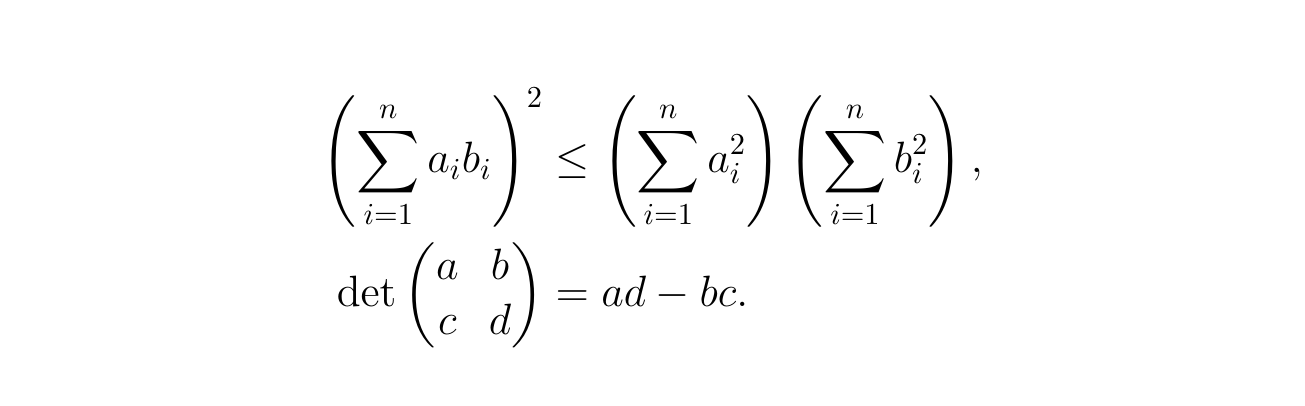
\includegraphics[width=.95\linewidth]{12a-formula-demo-input.png}}\\[-1mm]
  {\scriptsize\color{GOMuted}合成演示原图：柯西不等式与二阶行列式}
\end{minipage}\hfill
\begin{minipage}[t]{.66\linewidth}
  \fcolorbox{GOLine}{white}{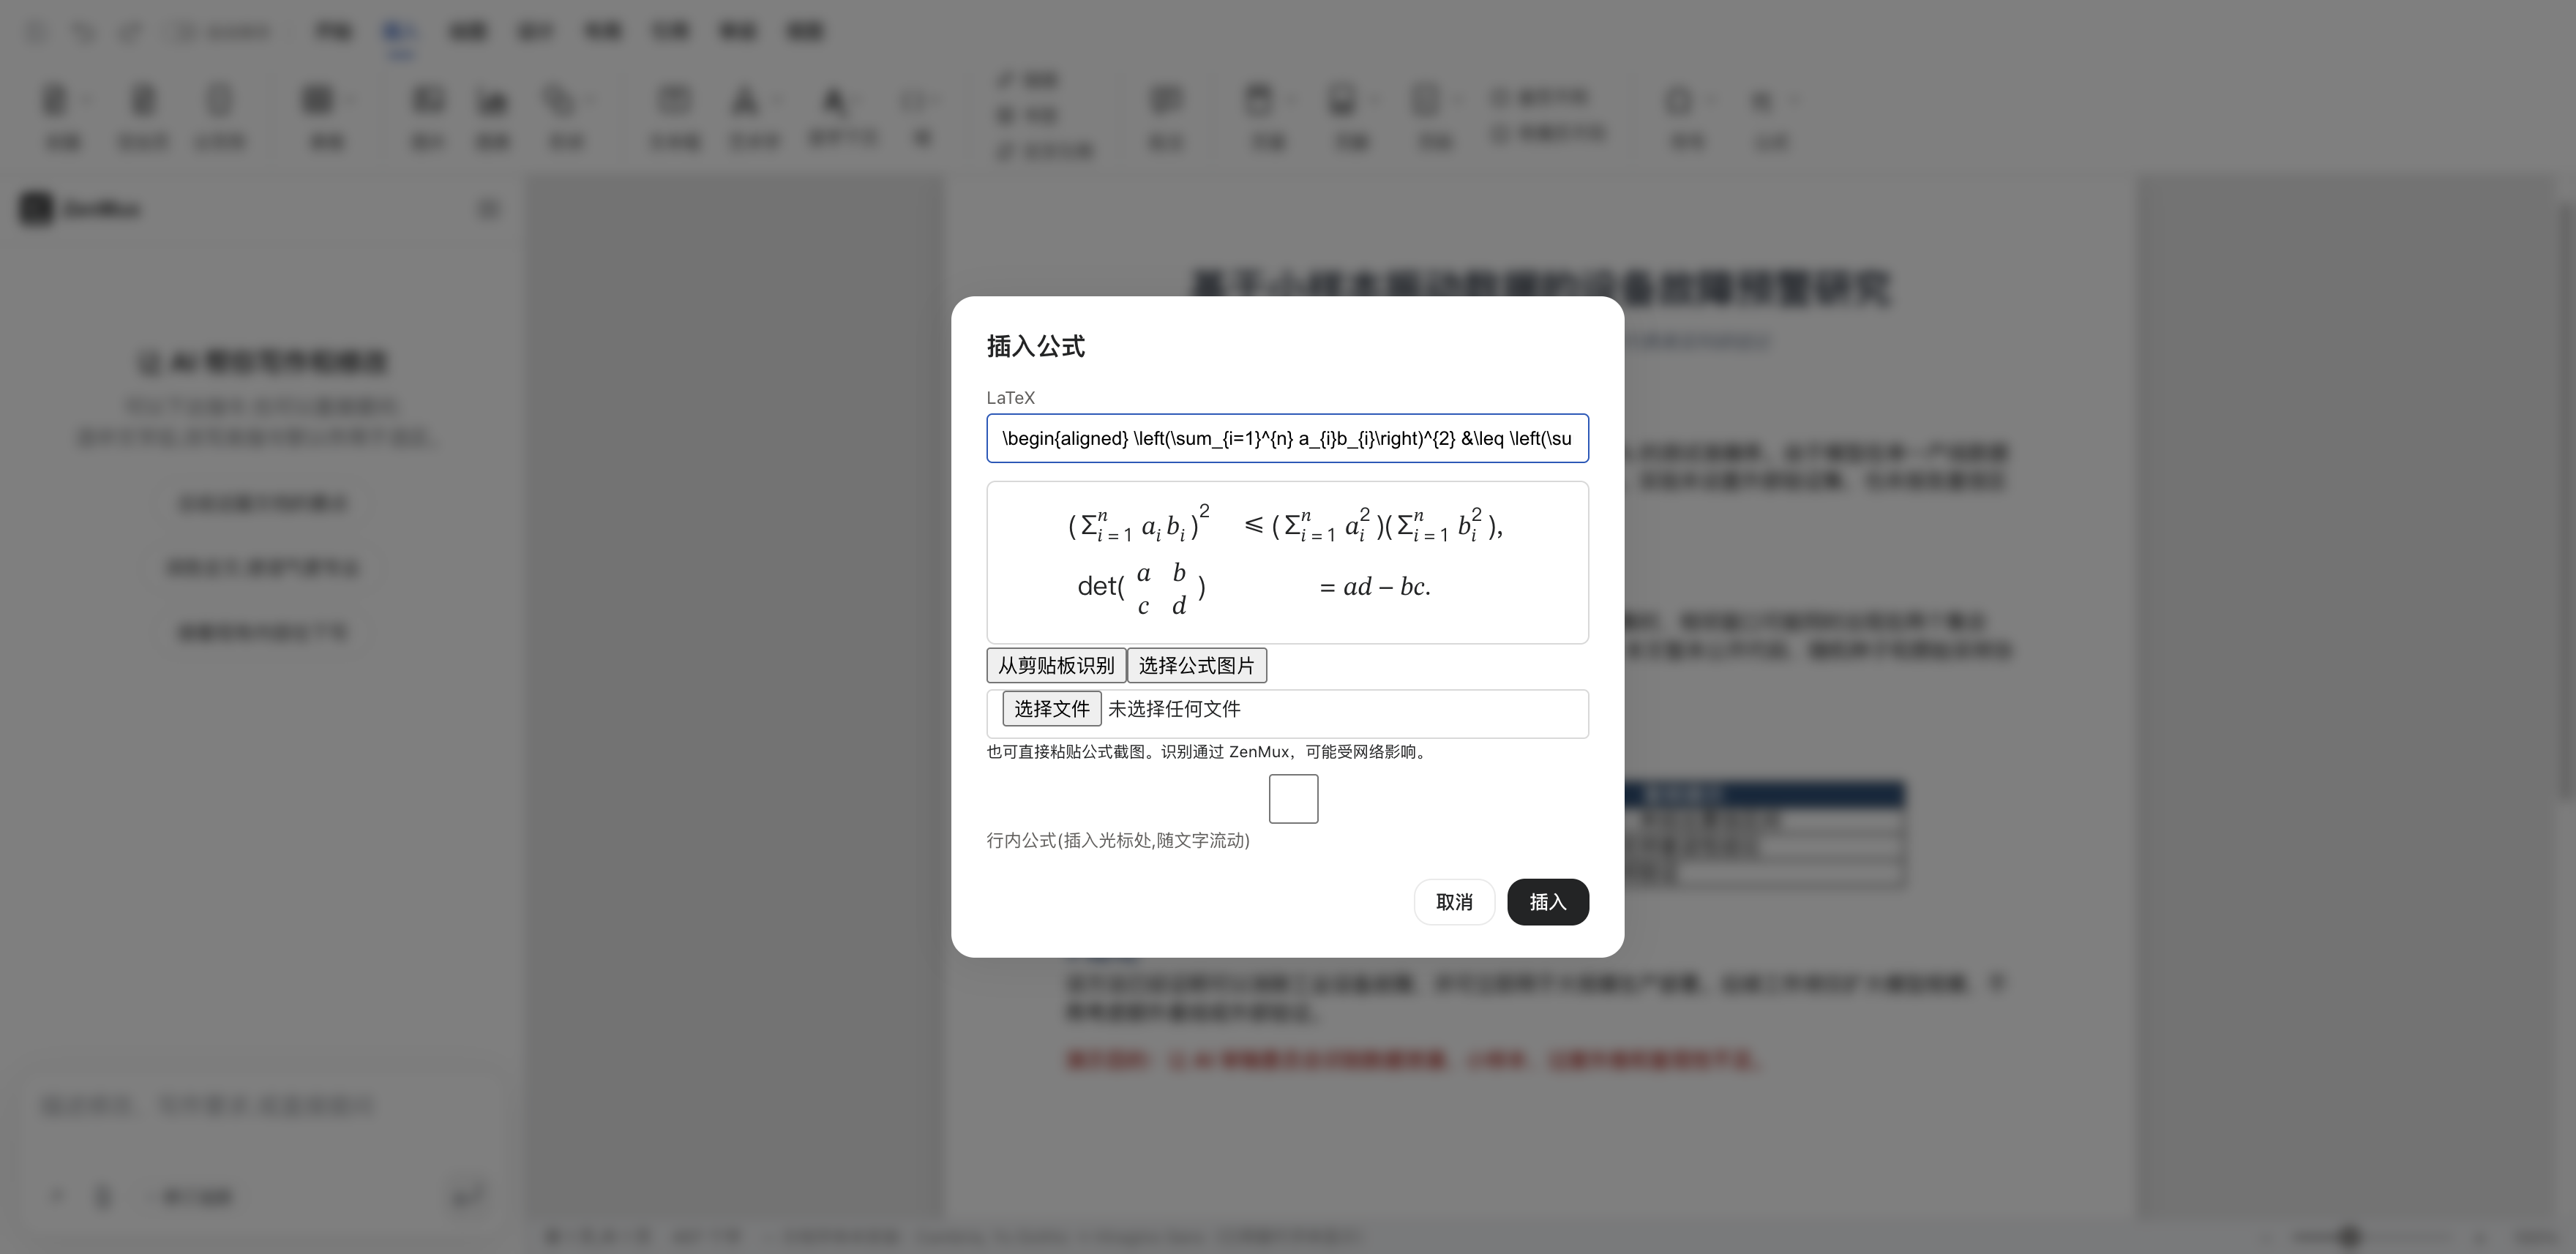
\includegraphics[width=.97\linewidth]{12-word-formula-recognition.png}}\\[-1mm]
  {\scriptsize\color{GOMuted}真实运行结果：LaTeX 源文与渲染预览同时可见}
\end{minipage}
\end{center}
\begin{enumerate}
  \item \textbf{0:00--0:30} 在 Word 打开“插入 > 公式 > 插入新公式”，粘贴截图或选择图片文件。
  \item \textbf{0:30--1:30} 等待 ZenMux 返回 LaTeX；逐项核对求和上下标、不等号、矩阵行列与换行。
  \item \textbf{1:30--2:30} 在预览中确认两行均正常渲染，点击“插入”；选择新公式并尝试修改一个符号。
  \item \textbf{2:30--3:00} 保存 DOCX、关闭再打开，确认公式仍是可编辑对象而非图片。
\end{enumerate}
\Tip{识别不准时先裁掉背景文字，只保留公式主体；不要直接把未经核对的 OCR 结果写进正式论文。}
}

\ENPage{A}{场景 A：公式截图变成 Word 可编辑公式}{Recipe A: turn a screenshot into an editable Word equation}{Send a paper screenshot to ZenMux vision, verify the LaTeX, then insert an equation object that remains editable in Word.}{
\begin{center}
\begin{minipage}[t]{.29\linewidth}
  \fcolorbox{GOLine}{white}{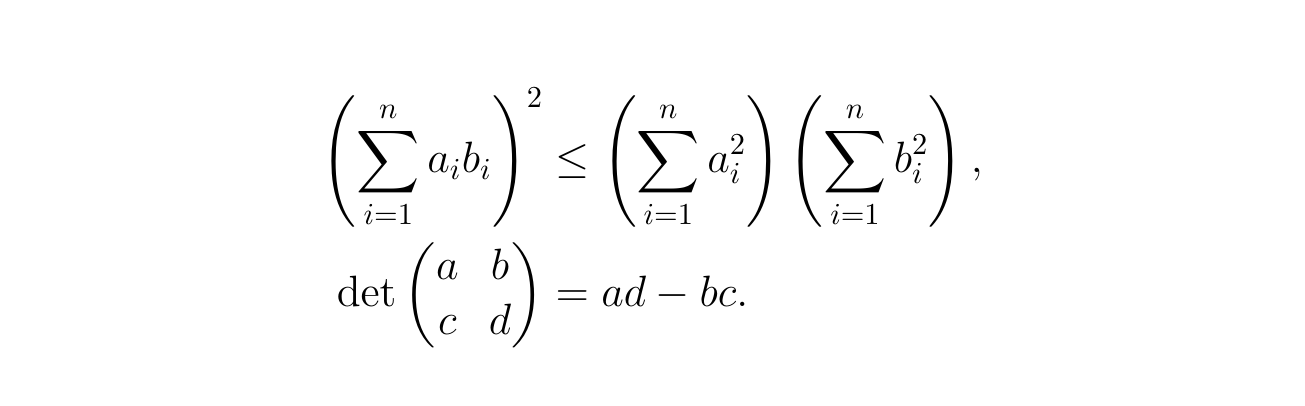
\includegraphics[width=.95\linewidth]{12a-formula-demo-input.png}}\\[-1mm]
  {\scriptsize\color{GOMuted}Synthetic input: Cauchy inequality and a $2\times2$ determinant}
\end{minipage}\hfill
\begin{minipage}[t]{.66\linewidth}
  \fcolorbox{GOLine}{white}{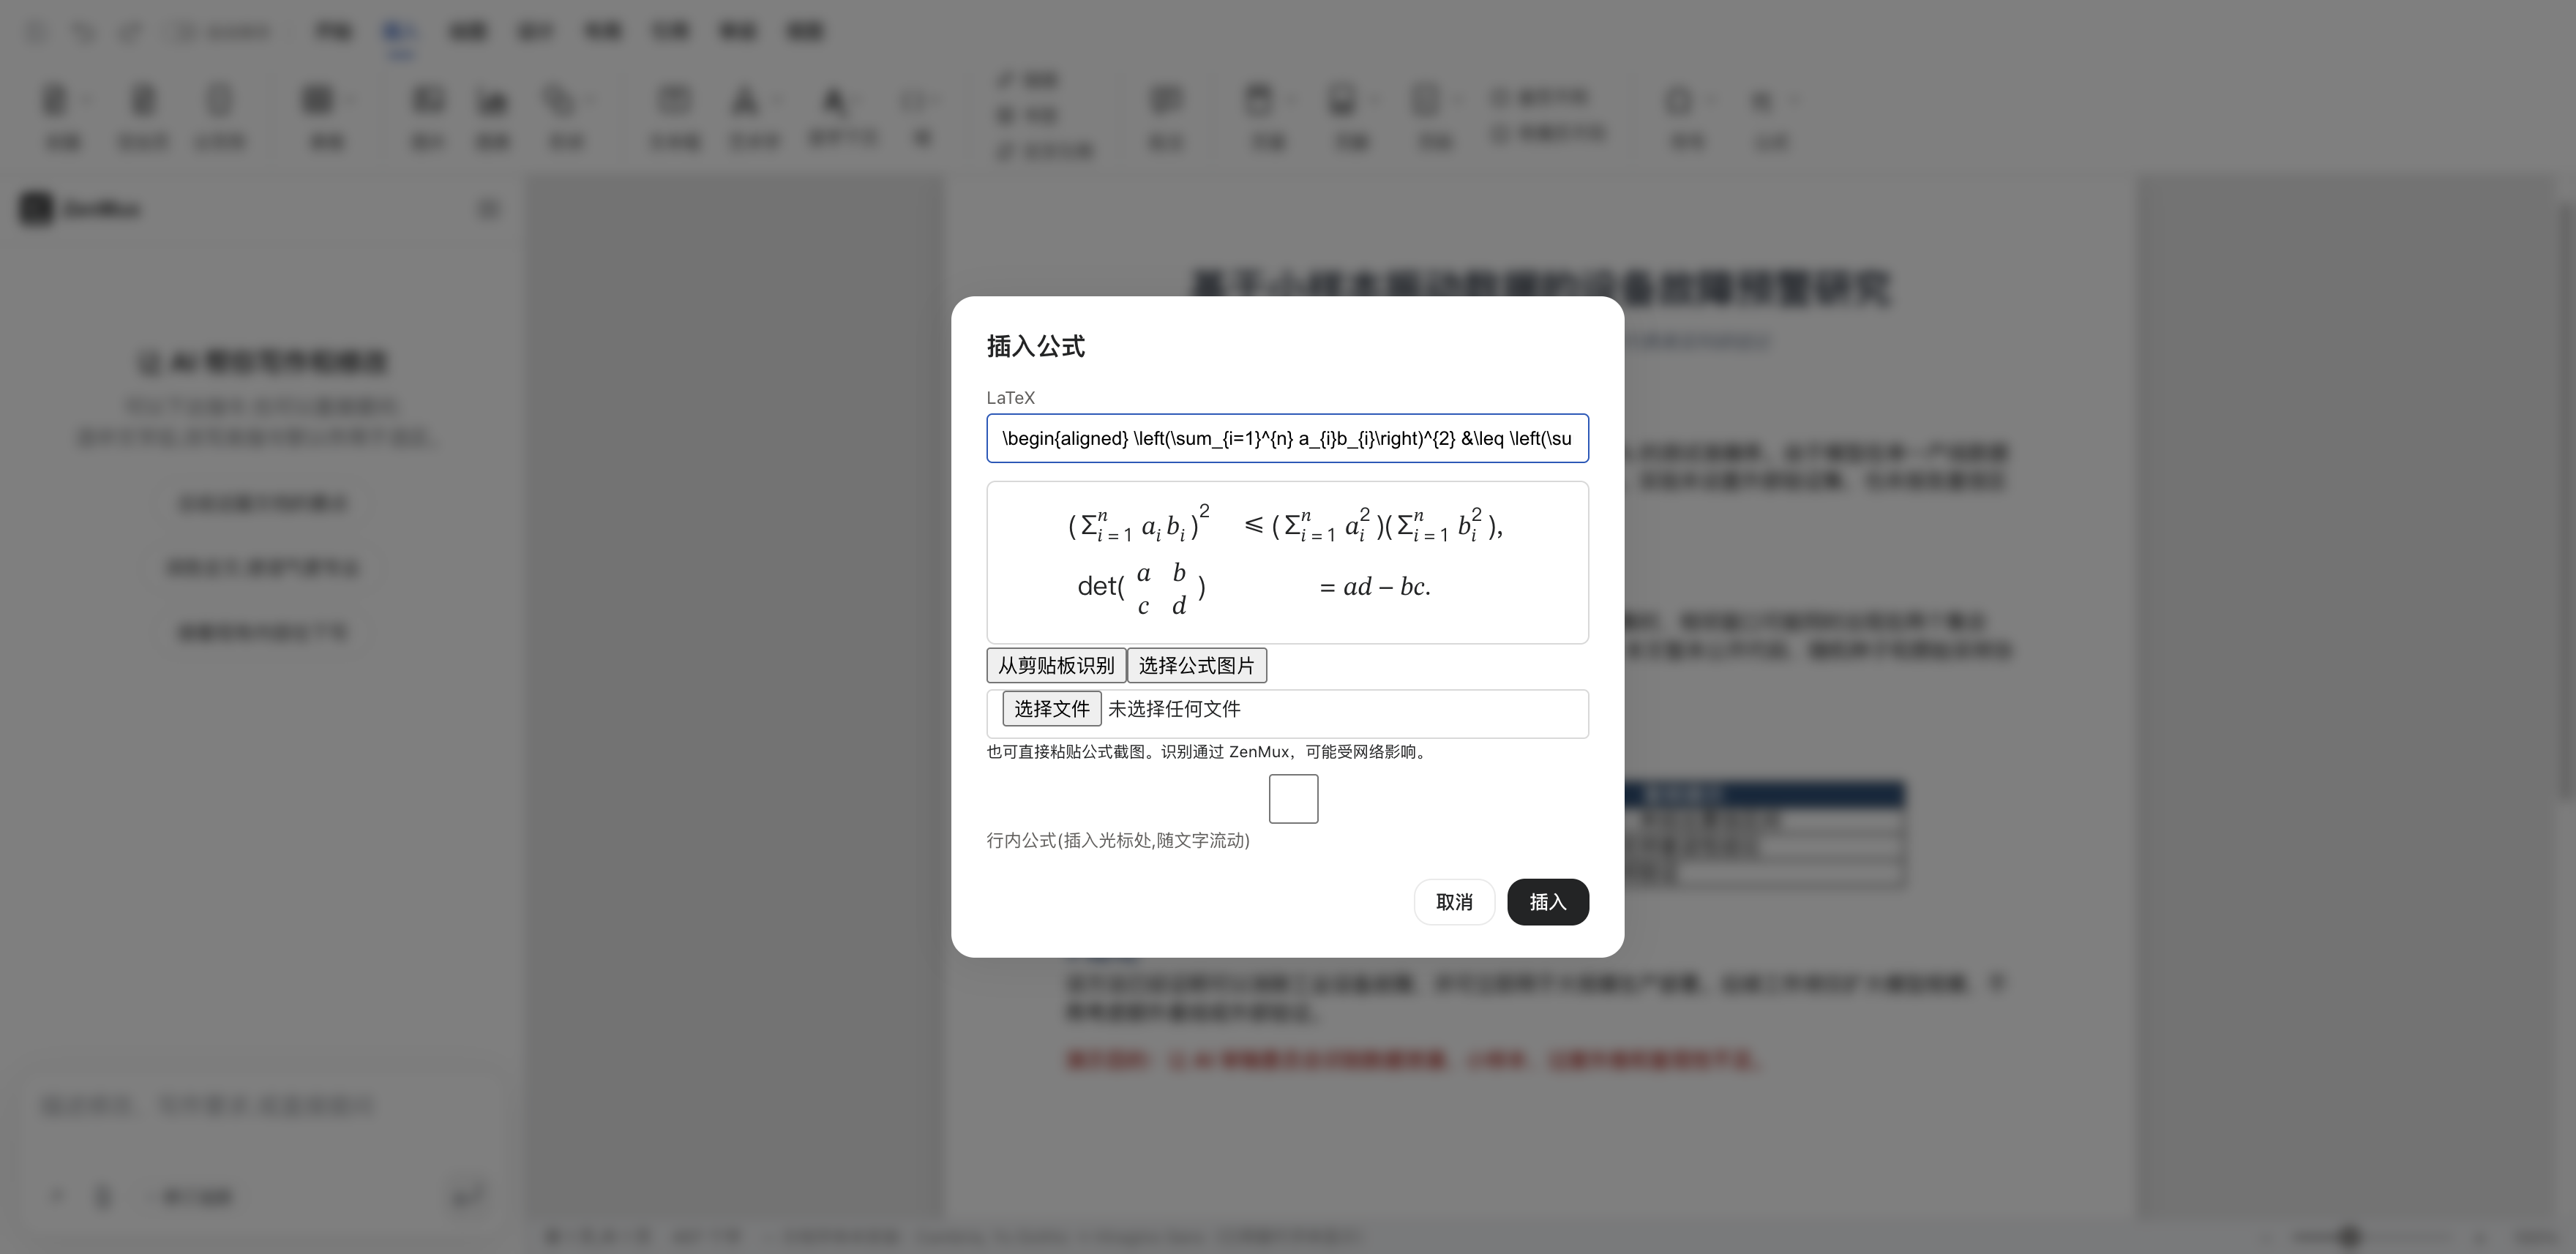
\includegraphics[width=.97\linewidth]{12-word-formula-recognition.png}}\\[-1mm]
  {\scriptsize\color{GOMuted}Real runtime result: editable LaTeX and rendered preview together}
\end{minipage}
\end{center}
\begin{enumerate}
  \item \textbf{0:00--0:30} In Word, open Insert > Equation > Insert new equation, then paste a capture or choose an image.
  \item \textbf{0:30--1:30} Wait for ZenMux and verify sums, indices, inequality signs, matrix rows, and line breaks.
  \item \textbf{1:30--2:30} Confirm both lines in preview, insert, select the new equation, and edit one symbol.
  \item \textbf{2:30--3:00} Save, close, and reopen the DOCX to confirm that the equation is not a bitmap.
\end{enumerate}
\Tip{If recognition is weak, crop away prose and keep only the equation. Never place unchecked OCR output in a final paper.}
}

\CNPage{B}{场景 B：Excel 一键完成图表与 EDA}{Recipe B: chart and EDA from an Excel table}{打开一份包含合成生产质量数据的真实 XLSX，让原生图表指出良品率骤降，再由 ZenMux 识别缺失值、重复行和联合异常。}{
\SmallShot{18-sheets-data-chart.png}{真实运行态：可编辑数据、中文原生折线图与人为注入的异常日同屏显示。}
\SmallShot{19-sheets-ai-anomaly-report.png}{真实 ZenMux 分析：指出缺失值、重复记录、异常阈值及产线改进建议。}
\begin{enumerate}
  \item \textbf{0:00--0:40} 打开 XLSX，确认字段、单位与“全部数据为合成示例”的提示。
  \item \textbf{0:40--1:30} 选择日期与良品率，插入折线图；用中文标题和轴标签说明问题。
  \item \textbf{1:30--2:30} 点击“AI 分析”，要求完整 EDA：缺失、重复、异常、趋势及证据行。
  \item \textbf{2:30--3:00} 对照第 18 个观测的 96.4°C、8.70 mm/s、17.8\% 缺陷率与 82.2\% 良品率，确认 AI 没有捏造。
\end{enumerate}
\Warn{此处数据为确定性合成演示，不对应任何企业。AI 建议必须结合业务规则、统计诊断和领域专家复核。}
}

\ENPage{B}{场景 B：Excel 一键完成图表与 EDA}{Recipe B: create a chart and EDA from an Excel table}{Open a real XLSX containing synthetic production-quality data, reveal the yield drop in a native chart, and ask ZenMux to find missing, duplicate, and jointly anomalous records.}{
\SmallShot{18-sheets-data-chart.png}{Real runtime: editable data, a Chinese native line chart, and the injected anomaly in one view.}
\SmallShot{19-sheets-ai-anomaly-report.png}{Real ZenMux analysis identifies missing data, the duplicate, anomaly thresholds, and improvement actions.}
\begin{enumerate}
  \item \textbf{0:00--0:40} Open the XLSX and verify fields, units, and the synthetic-data notice.
  \item \textbf{0:40--1:30} Select date and yield, insert a line chart, and give it clear title and axis labels.
  \item \textbf{1:30--2:30} Choose AI Analysis and request missing values, duplicates, anomalies, trends, and evidence rows.
  \item \textbf{2:30--3:00} Check observation 18: 96.4°C, 8.70 mm/s, 17.8\% defects, and 82.2\% yield. Reject any unsupported claim.
\end{enumerate}
\Warn{This is deterministic synthetic data, not a real company dataset. Combine AI suggestions with business rules, statistical diagnostics, and expert review.}
}

\CNPage{C}{场景 C：真实 DOI 变成 GB/T 7714 引用}{Recipe C: DOI to a GB/T 7714 citation}{用公开索引检索真实 DOI，把 AlphaFold 的 Nature 论文加入本地文献库，插入正文引文，并自动在文末生成参考文献。}{
\SmallShot{13-word-citation-search-results.png}{真实查询：OpenAlex/Crossref 返回 DOI 记录、OA/正式出版标签及 GB/T 7714 预览。}
\SmallShot{14-word-citation-bibliography.png}{真实写回：文末出现“参考文献”和完整 AlphaFold 条目。}
\begin{enumerate}
  \item \textbf{0:00--0:45} 打开“引用 > 科研文献”，选择 GB/T 7714，查询 \nolinkurl{10.1038/s41586-021-03819-2}。
  \item \textbf{0:45--1:30} 对照题名、作者、Nature、2021、卷页与 DOI，选择正确正式版本并导入。
  \item \textbf{1:30--2:20} 在正文输入 \texttt{/cite}，从本地条目列表选择；或直接点击记录旁“引用”。
  \item \textbf{2:20--3:00} 检查文末参考文献，导出 .bib，并把 DOCX 与 BIB 一起保存。
\end{enumerate}
\Tip{公开元数据也可能不完整；提交前以 DOI 落地页和期刊官网为准，并区分预印本与正式同行评审版本。}
}

\ENPage{C}{场景 C：真实 DOI 变成 GB/T 7714 引用}{Recipe C: turn a DOI into a GB/T 7714 citation}{Search public indexes for a real DOI, add the AlphaFold Nature article to the local library, insert an in-text citation, and generate the bibliography automatically.}{
\SmallShot{13-word-citation-search-results.png}{Real query: OpenAlex/Crossref metadata, DOI/OA/version badges, and a GB/T 7714 preview.}
\SmallShot{14-word-citation-bibliography.png}{Real write-back: References and the complete AlphaFold entry at the end of the document.}
\begin{enumerate}
  \item \textbf{0:00--0:45} Open References > Research literature, choose GB/T 7714, and query \nolinkurl{10.1038/s41586-021-03819-2}.
  \item \textbf{0:45--1:30} Verify title, authors, Nature, 2021, volume/pages, and DOI, then import the published version.
  \item \textbf{1:30--2:20} Type \texttt{/cite} and choose the local entry, or use Cite beside the search result.
  \item \textbf{2:20--3:00} Inspect the bibliography at the end, export .bib, and save DOCX and BIB together.
\end{enumerate}
\Tip{Public metadata can still be incomplete. Verify against the DOI landing page or journal and distinguish preprints from peer-reviewed versions.}
}

% =============================================================================
% PART II — Shared AI workflow
% =============================================================================
\PartPage{II}{选中、提问、流转：AI 工作流}{Select, ask, and route: the AI workflow}{五类编辑器共享上下文、附件、剪贴板、公式渲染、消息复制和 @Connect 信息通路。}{Five editors share context, attachments, clipboard input, equation rendering, message copy, and @Connect.}

\CNPage{07}{选择内容作为 AI 上下文}{Use selected content as AI context}{先选择，再提问，是最可靠的精确修改方式。Word 选择段落，Excel 选择单元格，PPT 选择对象，Markdown 选择文字；PDF 使用矩形框选页面区域。}{
\Flow{选择内容}{检查上下文卡}{向 ZenMux 提问}{审阅后写回}
\begin{enumerate}
  \item 在编辑器中完成选择，确认界面出现选区、对象、单元格范围或 PDF 区域缩略图。
  \item 提问时说明动作和边界，例如“只润色选中段落，不改变公式和引用键”。
  \item 先阅读 AI 回复或差异，再执行替换、插入或应用；不满意时撤销并缩小任务范围。
  \item Markdown 会冻结发送时的锚点；若用户随后修改原文，过期锚点会阻止错误回填。
\end{enumerate}
\Tip{没有选择时，AI 可能读取全文或当前页面。处理长文档时，显式选择能减少歧义、延迟和不必要的上下文。}
}

\ENPage{07}{选择内容作为 AI 上下文}{Use selected content as AI context}{Select first, then ask. Word selects paragraphs, Excel selects cells, PowerPoint selects objects, Markdown selects text, and PDF captures a rectangular page region.}{
\Flow{Select content}{Check context card}{Ask ZenMux}{Review and apply}
\begin{enumerate}
  \item Make the selection and confirm that the UI shows a range, object, text card, or PDF region thumbnail.
  \item State both action and boundary, for example: “Polish only the selected paragraph; preserve equations and citation keys.”
  \item Read the response or diff before replacing, inserting, or applying. Undo and narrow the task if the result is not acceptable.
  \item Markdown freezes the anchor at send time. If the source is edited later, a stale anchor is rejected to prevent misplaced write-back.
\end{enumerate}
\Tip{With no explicit selection, AI may use the full document or current page. Explicit context reduces ambiguity, latency, and unnecessary input on long files.}
}

\CNPage{08}{附件、图片与剪贴板}{Attachments, images, and clipboard}{AI 输入每次最多支持 5 个附件。文件可通过选择器或拖放添加；剪贴板图片会显示为可删除缩略图，并发送给视觉模型。}{
\begin{center}\begin{tikzpicture}
\foreach \x/\lab in {0/文件,2.2/图片,4.4/剪贴板,6.6/拖放,8.8/框选} {
  \node[draw=GOLine,fill=white,rounded corners=3pt,minimum width=1.8cm,minimum height=1.25cm,font=\small\bfseries] at (\x,0) {\lab};
}
\draw[GOBlue,very thick,-stealth] (9.8,0)--(11.2,0);
\node[fill=GOBlue,text=white,rounded corners=3pt,minimum width=2cm,minimum height=1.25cm,font=\small\bfseries] at (12.2,0) {ZenMux};
\end{tikzpicture}\end{center}
\begin{itemize}
  \item 普通文件会先在本机解析可读取内容；图片作为视觉输入。大型、加密或不受支持的文件可能无法解析。
  \item 用 Cmd/Ctrl+V 粘贴剪贴板图片；发送前检查缩略图，点击删除可移除不需要的附件。
  \item 附件总数超过 5 个时，先删除或分批提问。不要把 API Key、密码、未脱敏个人信息作为附件。
  \item 网络失败重试时，应用尽量保留原附件和框选内容；仍建议在重新发送前确认缩略图列表。
\end{itemize}
\Warn{发送附件会把相关内容交给所选 ZenMux 模型处理。涉及保密、伦理审查或受限数据时，先遵守所在机构政策。}
}

\ENPage{08}{附件、图片与剪贴板}{Attachments, images, and clipboard}{Each AI request accepts up to five attachments. Add files with the picker or drag-and-drop; pasted images appear as removable thumbnails and are sent as visual input.}{
\begin{center}\begin{tikzpicture}
\foreach \x/\lab in {0/File,2.2/Image,4.4/Clipboard,6.6/Drop,8.8/Region} {
  \node[draw=GOLine,fill=white,rounded corners=3pt,minimum width=1.8cm,minimum height=1.25cm,font=\small\bfseries] at (\x,0) {\lab};
}
\draw[GOBlue,very thick,-stealth] (9.8,0)--(11.2,0);
\node[fill=GOBlue,text=white,rounded corners=3pt,minimum width=2cm,minimum height=1.25cm,font=\small\bfseries] at (12.2,0) {ZenMux};
\end{tikzpicture}\end{center}
\begin{itemize}
  \item Ordinary files are parsed locally before relevant content is supplied; images are visual input. Large, encrypted, or unsupported files may not parse.
  \item Paste a clipboard image with Cmd/Ctrl+V. Check thumbnails before sending and remove any item that is not needed.
  \item If the total exceeds five, remove items or split the task. Never attach API Keys, passwords, or unredacted personal information.
  \item The app attempts to retain attachments and PDF regions after network failure. Confirm the thumbnail list again before retrying.
\end{itemize}
\Warn{Relevant attachment content is processed by the selected ZenMux model. Follow institutional rules before sending confidential, ethics-controlled, or otherwise restricted data.}
}

\CNPage{09}{复制消息并恢复文档 AI 历史}{Copy messages and restore file history}{Word、Excel、PowerPoint、Markdown、PDF 中，用户发出的提示词和 AI 回复都可以复制。问答按文件路径永久保存在本机，再次打开同一个文件会恢复最近 200 条消息。}{
\begin{itemize}
  \item 在消息旁使用复制按钮；粘贴到纯文本编辑器时得到源文，粘贴到支持富文本的目标时可保留适合的结构。
  \item 保存并关闭文档后，再次打开相同绝对路径的文件，AI 面板会显示“之前的对话”；恢复的历史也可以继续复制，并重新加入模型上下文。
  \item 历史只写入本机项目存储，不会进入文档正文、GitHub 仓库或安装包。若把文件另存到新路径，新副本会使用独立历史；原路径仍保留原会话。
  \item 行内公式使用 \texttt{\$...\$}，独立公式使用 \texttt{\$\$...\$\$}；多行公式可使用 \texttt{aligned}、\texttt{gathered} 等 LaTeX 环境。
  \item AI 回复中的 GFM 表格、列表、粗体和公式会统一解析；流式传输尚未闭合的定界符会暂时按可读文本显示，完成后再渲染。
  \item 若某段公式仍未渲染，先复制源文，检查反斜杠、成对定界符和下划线是否被意外转义。
\end{itemize}
\begin{center}
\fbox{\begin{minipage}{.9\linewidth}
行内：$E=mc^2$\qquad 多行：\(\begin{aligned}F&=ma\\E_k&=\tfrac12mv^2\end{aligned}\)\\[2mm]
源文可复制，渲染结果可阅读，插入文档后仍可继续编辑。
\end{minipage}}
\end{center}
\Tip{表格不适合表达长段推理。可要求 AI 使用“短表格 + 表格后解释”，提高 Word 与 Markdown 中的可读性。}
}

\ENPage{09}{复制消息并恢复文档 AI 历史}{Copy messages and restore file history}{Word, Excel, PowerPoint, Markdown, and PDF can copy both prompts and replies. Conversations persist locally by file path, and reopening the same file restores up to the latest 200 messages.}{
\begin{itemize}
  \item Use the copy control beside a message. A plain-text destination receives source; a rich destination can preserve suitable structure.
  \item Save and close the document, then reopen the exact same absolute path. The AI panel shows “Earlier messages”; restored items remain copyable and are returned to model context.
  \item History stays in local project storage. It is not written into document content, the GitHub repository, or an installer. Save As to a new path creates an independent history while the original path retains its conversation.
  \item Use \texttt{\$...\$} for inline math and \texttt{\$\$...\$\$} for display math. Multiline equations can use LaTeX environments such as \texttt{aligned} or \texttt{gathered}.
  \item GFM tables, lists, emphasis, and equations share the same reply parser. An unclosed delimiter remains readable during streaming and renders when complete.
  \item If a formula does not render, copy the source and check backslashes, paired delimiters, and accidentally escaped underscores.
\end{itemize}
\begin{center}
\fbox{\begin{minipage}{.9\linewidth}
Inline: $E=mc^2$\qquad Multiline: \(\begin{aligned}F&=ma\\E_k&=\tfrac12mv^2\end{aligned}\)\\[2mm]
Source remains copyable, rendering remains readable, and inserted equations remain editable.
\end{minipage}}
\end{center}
\Tip{A wide table is a poor container for long reasoning. Ask for a concise table followed by prose to improve readability in Word and Markdown.}
}

\CNPage{10}{跨编辑器联动：用 @Connect 一键流转 AI 结果}{Cross-editor routing: send AI results with @Connect}{在 AI 输入中键入 @Connect，可把最近一条 AI 回复送到另一个已经打开的 Word、Excel、PPT 或 Markdown 标签页。源可以来自五类编辑器，包括 PDF。}{
\AppStrip
\begin{enumerate}
  \item 先打开目标文件，确保目标标签页已经出现在 ZenOffice 窗口中。
  \item 在当前 AI 输入框键入 \texttt{@Connect}，从正确的开放标签列表中选择目标；不要仅凭相似文件名判断。
  \item 发送后检查目标：Word/Markdown 接收可编辑文本，Excel 接收适合单元格的内容，PPT 接收可编辑文本框，而不是扁平截图。
  \item 连接只在本机应用内部传递回复；目标文件仍需用户保存。若目标关闭或改名，重新打开后再选择。
\end{enumerate}
\Tip{推荐工作流：PDF 框选提问 $\rightarrow$ @Connect 到 Word 整理；Excel 分析 $\rightarrow$ @Connect 到 PPT 形成汇报提纲。}
}

\ENPage{10}{跨编辑器联动：用 @Connect 一键流转 AI 结果}{Cross-editor routing: send AI results with @Connect}{Type @Connect in an AI input to send the latest reply to another open Word, Excel, PowerPoint, or Markdown tab. The source can be any of the five editors, including PDF.}{
\AppStrip
\begin{enumerate}
  \item Open the destination first and confirm that its tab is visible in ZenOffice.
  \item Type \texttt{@Connect}, then choose the correct item from the list of open targets. Do not rely only on similar filenames.
  \item Verify the destination: Word/Markdown receives editable text, Excel receives cell-suitable content, and PowerPoint receives an editable text box rather than a flattened screenshot.
  \item Transfer is local to the app, but the destination file still needs to be saved. If a target is closed or renamed, reopen it before selecting again.
\end{enumerate}
\Tip{Useful flows: PDF region question $\rightarrow$ @Connect to Word for synthesis; Excel analysis $\rightarrow$ @Connect to PowerPoint for a briefing outline.}
}

% =============================================================================
% PART III — Word
% =============================================================================
\PartPage{III}{Word：从写作到投稿预审}{Word: from draft to pre-submission review}{编辑真实 DOCX，处理分页、样式、图片环绕、公式、文献、审稿与 AI 配图。}{Edit real DOCX files with pagination, styles, image wrapping, equations, citations, review, and AI imagery.}

\CNPage{11}{创建、打开与保存 DOCX}{Create, open, and save DOCX}{Word 工作台直接处理 DOCX。未修改的文档部分尽量保持原始结构；保存前仍应检查页面、字体、图片和复杂对象。}{
\Shot{05-word-editor.png}{当前源码真实运行态：Word 编辑器、分页画布、功能区与左侧 ZenMux AI 面板。}
\begin{itemize}
  \item 从主页点击 AI Docs 新建，或用“打开本地文件”选择 .docx/.doc。标题栏显示当前文件名与保存状态。
  \item 打开旧版 .doc 时，应用优先调用本机 LibreOffice 转换为独立 DOCX；若不可用，则使用纯 JavaScript 文字恢复兜底。转换结果另存为新文件，绝不覆盖原始 .doc。
  \item 使用 Cmd/Ctrl+S 保存，Cmd/Ctrl+Shift+S 另存。首次保存的新文档需要选择位置与文件名。
  \item 自动保存可减少意外损失，但在大幅修改前仍建议另存版本；关闭时留意未保存提示。
  \item 在 Microsoft Word 或其他兼容应用中复核交付文件，尤其是特殊字体、域、目录、浮动对象和跨页表格。
\end{itemize}
\Tip{旧版 DOC 的复杂版式、嵌入对象或宏可能无法完整转换。处理重要文件时，保留“原始文件、转换后的 DOCX、最终交付”三份。}
}

\ENPage{11}{创建、打开与保存 DOCX}{Create, open, and save DOCX}{The Word workspace edits real DOCX files. Unchanged areas are preserved as narrowly as possible, but page layout, fonts, images, and complex objects still deserve a final check.}{
\Shot{05-word-editor.png}{Real runtime UI: Word editor, paginated canvas, ribbon, and the ZenMux AI panel on the left.}
\begin{itemize}
  \item Choose AI Docs to create a file or Open local file to select a .docx/.doc. The title area shows filename and save state.
  \item For legacy .doc, ZenOffice first asks local LibreOffice for a high-fidelity conversion to a separate DOCX. If unavailable, a pure-JavaScript text-recovery path is used. The original .doc is never overwritten.
  \item Use Cmd/Ctrl+S to save and Cmd/Ctrl+Shift+S for Save As. A new document asks for location and name on first save.
  \item Auto-save reduces accidental loss, but create a new version before major edits and respond to unsaved-close prompts.
  \item Review deliverables in Microsoft Word or another compatible app, especially custom fonts, fields, contents, floating objects, and multipage tables.
\end{itemize}
\Tip{Complex legacy layout, embedded objects, or macros may not convert completely. Keep the untouched DOC, converted DOCX, and final delivery as separate files.}
}

\CNPage{12}{文字、段落、样式与 AI 修改}{Text, paragraphs, styles, and AI edits}{功能区用于字体、字号、粗斜体、颜色、对齐、列表和样式。选择一段文字后，AI 可以只针对选区润色、翻译、总结或改写。}{
\SmallShot{05-word-editor.png}{Word 真实运行态：文字编辑区和 ZenMux AI 面板并排，便于先选中再提问。}
\begin{enumerate}
  \item 先选择文字，再调整字体或字号；若字号输入不顺畅，可点击字号框、全选数值、输入目标大小并按 Enter。
  \item 用样式而不是逐段手工放大来建立标题层级；列表、缩进和段前段后距应通过段落工具统一设置。
  \item AI 修改时写清楚语言、语气、长度和禁止改变项，例如“保持数字、LaTeX 公式、引用键和专有名词不变”。
  \item 应用前查看差异；应用后用撤销检查可恢复性。跨多个段落时分批处理，减少格式被连带改变。
\end{enumerate}
\Tip{长文档先统一样式，再让 AI 润色正文。这样内容修改和版式修改更容易分别审阅。}
}

\ENPage{12}{文字、段落、样式与 AI 修改}{Text, paragraphs, styles, and AI edits}{The ribbon controls font, size, emphasis, color, alignment, lists, and styles. After selecting text, AI can polish, translate, summarize, or rewrite only that range.}{
\SmallShot{05-word-editor.png}{Real Word runtime: editing surface beside the ZenMux panel, designed for select-then-ask work.}
\begin{enumerate}
  \item Select text before changing font or size. If the size control feels awkward, focus it, select the current value, type the target, and press Enter.
  \item Build hierarchy with styles rather than manually enlarging every heading. Use paragraph controls for lists, indents, and spacing.
  \item State language, tone, length, and protected items: “Preserve numbers, LaTeX equations, citation keys, and proper nouns.”
  \item Review the diff before applying and test Undo afterward. Split a large multi-paragraph change into smaller batches to limit format side effects.
\end{enumerate}
\Tip{Normalize styles before polishing a long manuscript. Content and layout changes then remain easier to review separately.}
}

\CNPage{13}{插入图片与文字环绕}{Insert images and wrap text}{图片可从文件、剪贴板或拖放进入 Word，并支持嵌入、四周、紧密、穿越、上下、衬于文字下方及浮于文字上方等布局。}{
\SmallShot{06-word-insert.png}{当前源码真实运行态：Word“插入”功能区中的图片、表格、公式与绘图入口。}
\begin{enumerate}
  \item 在“插入”中选择图片，或把本地图片拖到文档目标位置。插入后先确认图片仍在页面边界内。
  \item 选择环绕方式：正文中的内容优先用“嵌入”；需要自由布局时使用四周/紧密；背景图或水印式素材才使用衬于文字下方。
  \item 通过角点等比缩放；宽高可输入并实时更新。自由浮动图片要检查锚点、层级和跨页位置。
  \item 导出 PDF 前使用分页预览检查图像尺寸、页面纸张、边距和是否出现边框；导出结果应与页面画布 1:1 对应。
\end{enumerate}
\Warn{浮于文字上方或下方时若图片看似消失，先检查层级、锚点所在页、页面边界和缩放比例，再撤销最近一次布局操作。}
}

\ENPage{13}{插入图片与文字环绕}{Insert images and wrap text}{Images can enter Word from a file, clipboard, or drag-and-drop. Layout modes include inline, square, tight, through, top and bottom, behind text, and in front of text.}{
\SmallShot{06-word-insert.png}{Real runtime UI: Word Insert ribbon with image, table, equation, and drawing entry points.}
\begin{enumerate}
  \item Choose Picture under Insert or drop a local image at the intended location. Confirm that the object remains inside the page boundary.
  \item Prefer Inline for body content. Use square/tight for controlled floating layout; reserve Behind text for background-like material.
  \item Resize proportionally from a corner. Width and height fields update the object; for floating images, verify anchor, z-order, and page position.
  \item Before PDF export, compare paginated preview, paper size, margins, image dimensions, and borders. The exported page should match the canvas one-to-one.
\end{enumerate}
\Warn{If an image appears to vanish in front-of-text or behind-text mode, check z-order, anchor page, page bounds, and zoom, then undo the most recent layout change.}
}

\CNPage{14}{一张截图变成可编辑 LaTeX 公式}{Turn a screenshot into editable LaTeX}{Word 支持行内和独立公式、多行环境，以及从剪贴板截图或图片文件识别公式。识别结果先以 LaTeX 文本确认，再按文档公式形式插入。}{
\SmallShot{12-word-formula-recognition.png}{真实 ZenMux 识别：柯西不等式与二阶行列式的 LaTeX 源文和渲染预览。}
\begin{itemize}
  \item 行内公式适合句中变量，如 \(F=ma\)；独立公式适合推导与编号。多行可使用 \texttt{aligned}：
\end{itemize}
\[
\begin{aligned}
  F &= ma,\\
  E_k &= \frac{1}{2}mv^2.
\end{aligned}
\]
\begin{enumerate}
  \item 从“插入 > 公式”输入 LaTeX，预览后插入。需要修改时选择公式对象，再进入编辑。
  \item 识别图片公式时，可粘贴截图或选择图片文件；裁剪应只保留公式和必要编号，避免背景文字干扰。
  \item 核对上下标、希腊字母、分式、矩阵、对齐点和多行换行；AI OCR 对低清晰度或手写公式可能误判。
  \item 保存并在 Word 中复核公式是否仍为可编辑对象，而不是普通截图。
\end{enumerate}
\Tip{复杂公式建议同时保留一份 LaTeX 源文，便于在 Word、PPT、Excel 与 Markdown 之间复用。}
}

\ENPage{14}{一张截图变成可编辑 LaTeX 公式}{Turn a screenshot into editable LaTeX}{Word supports inline and display equations, multiline environments, and recognition from clipboard captures or image files. Confirm the recognized source before insertion.}{
\SmallShot{12-word-formula-recognition.png}{Real ZenMux recognition: LaTeX source and rendered preview for the Cauchy inequality and a determinant.}
\begin{itemize}
  \item Inline math suits variables in a sentence, such as \(F=ma\); display math suits derivations and numbered results. Use \texttt{aligned} for multiple lines:
\end{itemize}
\[
\begin{aligned}
  F &= ma,\\
  E_k &= \frac{1}{2}mv^2.
\end{aligned}
\]
\begin{enumerate}
  \item Enter LaTeX under Insert > Equation, preview, and insert. To revise, select the equation object before opening the editor.
  \item For image recognition, paste a screenshot or choose a file. Crop to the formula and necessary number so background prose does not interfere.
  \item Verify subscripts, superscripts, Greek letters, fractions, matrices, alignment points, and line breaks. Low-resolution or handwritten math may be misread.
  \item Save and verify in Word that the result remains an editable equation rather than a screenshot.
\end{enumerate}
\Tip{Keep a LaTeX source copy for complex formulas so the same math can be reused in Word, PowerPoint, Excel, and Markdown.}
}

\CNPage{15}{一键找到真文献并生成规范引用}{Find real literature and generate a complete citation}{Word 的“引用”入口可检索公开学术元数据、导入本地文献库、插入正文引用，并在文末生成参考文献表与 BibTeX 文件。}{
\SmallShot{13-word-citation-search-results.png}{真实 DOI 检索：AlphaFold Nature 论文、来源标签和 GB/T 7714 引用预览。}
\SmallShot{14-word-citation-bibliography.png}{真实写回：文末自动生成参考文献条目，正文与本地文献库保持关联。}
\begin{enumerate}
  \item 在“引用 > 科研文献”检索 OpenAlex、Crossref、Semantic Scholar、Europe PMC/PubMed 与 arXiv；受限平台会在浏览器打开官方搜索，不做不合规抓取。
  \item 将结果加入本地文献库，或导入 BibTeX、RIS、CSL-JSON。用 DOI、PMID、arXiv ID 检查重复，并区分预印本与正式发表版本。
  \item 在正文输入 \texttt{/cite}，从本地文献条目列表选择；也可从引用管理器插入。选择 GB/T 7714、APA 7、IEEE、Nature 或 Vancouver 样式。
  \item 完成后执行“插入参考文献表”，把条目写到文末；同时导出 .bib，即使只是临时交换文件也应保留到确认交付后。
\end{enumerate}
\Warn{元数据来自公开索引并不等于全文可合法下载。优先使用 OA 版本，并人工核对作者、题名、年份、期刊、卷期页和 DOI。}
}

\ENPage{15}{一键找到真文献并生成规范引用}{Find real literature and generate a complete citation}{Word References searches public scholarly metadata, imports a local library, inserts in-text citations, and generates both a bibliography and BibTeX.}{
\SmallShot{13-word-citation-search-results.png}{Real DOI query: the AlphaFold Nature article, provenance badges, and GB/T 7714 preview.}
\SmallShot{14-word-citation-bibliography.png}{Real write-back: a bibliography entry appears at the end and remains linked to the local library.}
\begin{enumerate}
  \item Search OpenAlex, Crossref, Semantic Scholar, Europe PMC/PubMed, and arXiv. Restricted services open official browser searches instead of being scraped.
  \item Add results to the local library or import BibTeX, RIS, or CSL-JSON. Deduplicate by DOI, PMID, or arXiv ID and distinguish preprints from published versions.
  \item Type \texttt{/cite} and choose from the local entry list, or insert through the manager. Select GB/T 7714, APA 7, IEEE, Nature, or Vancouver style.
  \item Insert Bibliography when drafting is complete so entries appear at the end, then export .bib and keep even a temporary exchange file until delivery is verified.
\end{enumerate}
\Warn{Public metadata does not imply that every full text can be downloaded lawfully. Prefer open-access copies and verify authors, title, year, journal, volume, pages, and DOI.}
}

\CNPage{16}{论文防拒稿利器：3 委员 + 1 主席严苛预审}{Reduce avoidable rejection: a three-reviewer committee plus chair}{审阅功能按文档类型建立 3 名独立委员和 1 名主席；模型从当前可用文本模型中分配，并可输出中文或英文审稿意见。}{
\SmallShot{15-word-ai-review-chair.png}{真实 Science 级演示：主席汇总三位委员意见，给出 Reject 结论、5/5 置信度与结构性问题。}
\SmallShot{17-word-ai-review-members.png}{真实委员报告：独立问题清单、作者问题与结论依据可逐项展开。}
\begin{itemize}
  \item 可选标准包括 Science、Nature、Cell、Elsevier、IEEE 顶刊、IEEE 顶级会议、IEEE 一般会议，以及国家自然科学基金、863、科技和商业标书等。
  \item 委员分别检查新颖性、方法、证据、统计、可复现性、表达和合规性；主席综合冲突意见、主要问题、次要问题与建议结论。
  \item 审阅范围包括正文、公式、表格、图片、图表和图形。视觉内容应清晰，且图注、编号和正文引用要完整。
  \item 选择报告语言后再开始；长文档可能耗时并受网络影响。保存审稿报告，同时把每条意见映射到具体页、段落、公式或图号。
\end{itemize}
\Warn{AI 审稿不是正式同行评议、基金评审或法律意见。随机模型分配不能替代领域专家，关键结论必须人工复核。}
}

\ENPage{16}{论文防拒稿利器：3 委员 + 1 主席严苛预审}{Reduce avoidable rejection: a three-reviewer committee plus chair}{Review creates three independent members plus a chair. Models are assigned from the available text-model list, and the report can be Chinese or English.}{
\SmallShot{15-word-ai-review-chair.png}{Real Science-level demonstration: the chair synthesizes three reports into a Reject decision and 5/5 confidence.}
\SmallShot{17-word-ai-review-members.png}{Real member output: independent concerns, questions for authors, and evidence for the verdict.}
\begin{itemize}
  \item Standards include Science, Nature, Cell, Elsevier, top IEEE journals, top IEEE conferences, general IEEE conferences, and several Chinese grant, 863, technology, and commercial proposal types.
  \item Members assess novelty, methods, evidence, statistics, reproducibility, writing, and compliance. The chair reconciles conflicts and separates major issues, minor issues, and recommendation.
  \item Scope includes prose, equations, tables, images, charts, and shapes. Visuals need adequate resolution plus complete captions, numbering, and textual references.
  \item Choose report language before starting. Long documents take time and depend on network conditions. Save the report and map every comment to a page, paragraph, equation, or figure.
\end{itemize}
\Warn{AI review is not formal peer review, grant adjudication, or legal advice. Random model assignment does not replace domain experts; verify every consequential conclusion.}
}

\CNPage{17}{AI 配图与扫描件处理}{AI imagery and scanned-page processing}{Word 配图通过 ZenMux 图像模型生成，默认适配文档比例。扫描件工具可保守增强黑白材料，或去除覆盖在印刷内容上的手写痕迹。}{
\SmallShot{06-word-insert.png}{Word“插入”运行态：本地图片与 AI 配图从同一文档工作流进入。}
\begin{enumerate}
  \item 生成配图时描述主题、构图、受众、比例、是否需要文字以及禁止出现的元素。Word 默认适合约 3:2 的文档配图。
  \item 去手写时选择包含原始扫描图的对象，使用 \texttt{openai/gpt-image-2} 处理；提示应要求保留印刷体、公式、表格、线条和纸张结构。
  \item 手写可能覆盖印刷字时，工具只应依据邻近笔画保守修复，不应臆造无法判断的内容。增强模式不等于去手写模式。
  \item 对比处理前后预览，放大核对数字、符号、签章和边缘；确认后才替换原图，并保留原始文件。
\end{enumerate}
\Warn{图像生成与修复具有不确定性，也可能受网络影响。涉及证据、档案、签字或科研原始记录时，不要用 AI 结果替代原件。}
}

\ENPage{17}{AI 配图与扫描件处理}{AI imagery and scanned-page processing}{Word illustrations are generated through ZenMux and use a document-friendly aspect ratio. Scan tools can conservatively enhance monochrome material or remove handwriting over printed content.}{
\SmallShot{06-word-insert.png}{Real Word Insert runtime: local images and AI illustrations enter the same document workflow.}
\begin{enumerate}
  \item Describe subject, composition, audience, aspect ratio, desired text, and prohibited elements. Word defaults to an illustration near a 3:2 document ratio.
  \item For handwriting removal, select the scanned image and use \texttt{openai/gpt-image-2}. Instruct it to preserve print, equations, tables, lines, and paper structure.
  \item Where handwriting overlaps print, reconstruction should be conservative and based only on nearby strokes. Enhancement mode is distinct from handwriting-removal mode.
  \item Compare before and after at high zoom, checking digits, symbols, stamps, and edges. Replace only after confirmation and retain the untouched original.
\end{enumerate}
\Warn{Image generation and restoration are uncertain and network-dependent. Never replace evidentiary, archival, signed, or original research records with an AI-processed image.}
}

% =============================================================================
% PART IV — Excel
% =============================================================================
\PartPage{IV}{Excel：从原始数据到可信结论}{Excel: from raw data to defensible findings}{在真实 XLSX 中完成公式、清洗、统计分析、字段驱动可视化和选区 AI 操作。}{Work in real XLSX files with formulas, cleaning, statistics, field-driven visualization, and selection-aware AI.}

\CNPage{18}{工作簿、工作表与基础编辑}{Workbooks, sheets, and basic editing}{Excel 工作台用于真实 XLSX 的打开、编辑和保存，支持公式重算、排序筛选、数据验证、条件格式、透视表及常见工作簿结构。}{
\Shot{09-sheets-editor.png}{当前源码真实运行态：Excel 工作台、网格、公式栏、功能区与 ZenMux AI 面板。}
\begin{itemize}
  \item 点击 AI Sheets 新建，或打开 .xlsx/.xls/.csv。导入 CSV 时先确认编码、分隔符、日期与小数点格式。
  \item 通过名称框或鼠标选择范围；公式以等号开始。粘贴前确认目标范围大小，避免覆盖邻近数据。
  \item 排序和筛选前确保表头唯一且没有不必要的合并单元格；数据验证适合限制类别、日期或数值范围。
  \item 保存后在 Excel 或兼容应用中复核公式结果、图表、透视表、打印区域和冻结窗格。
\end{itemize}
\Tip{分析前复制原始数据工作表，只在副本上清洗。保留一个“数据字典”工作表说明字段、单位、缺失值和来源。}
}

\ENPage{18}{工作簿、工作表与基础编辑}{Workbooks, sheets, and basic editing}{The Excel workspace opens, edits, and saves real XLSX files with formula recalculation, sorting, filtering, validation, conditional formatting, pivots, and common workbook structure.}{
\Shot{09-sheets-editor.png}{Real runtime UI: Excel grid, formula bar, ribbon, and ZenMux AI panel.}
\begin{itemize}
  \item Choose AI Sheets or open .xlsx/.xls/.csv. For CSV, verify encoding, delimiter, date conventions, and decimal separators.
  \item Select a range by mouse or name box; formulas begin with an equals sign. Confirm destination dimensions before pasting so adjacent data is not overwritten.
  \item Before sort/filter, use unique headers and avoid unnecessary merged cells. Validation is useful for categories, dates, and numeric limits.
  \item After saving, verify results in Excel or a compatible app, including formulas, charts, pivots, print area, and frozen panes.
\end{itemize}
\Tip{Duplicate the raw-data sheet and clean only the copy. Keep a data-dictionary sheet describing fields, units, missing values, and sources.}
}

\CNPage{19}{从原始数据到可信结论：完整 EDA}{From raw data to defensible findings: complete EDA}{选中已有字段后，从数据质量与描述统计开始，再进入相关、回归、时间序列、分组汇总、异常值或情景分析。}{
\SmallShot{19-sheets-ai-anomaly-report.png}{真实 ZenMux EDA：依据当前表格指出联合异常、缺失值、重复行和可执行的数据治理建议。}
\Flow{确认字段与单位}{检查缺失/异常}{选择分析方法}{验证并解释}
\begin{enumerate}
  \item 明确问题与分析单位；确认每行代表什么、每列类型、样本范围、时间频率和缺失值编码。
  \item 先做数据质量检查与描述统计，再决定相关、协方差、回归、分组比较、时间趋势、预测或异常检测。
  \item 把结果输出到新区域或新工作表，不覆盖原数据；记录筛选条件、参数与随机性。
  \item 检查模型假设、样本量、离群点和数据泄漏。相关不等于因果，预测区间比单点预测更重要。
\end{enumerate}
\Warn{AI 可以建议方法和生成步骤，但不能替代研究设计、统计诊断或领域判断。重要结论应由专业人员复核。}
}

\ENPage{19}{从原始数据到可信结论：完整 EDA}{From raw data to defensible findings: complete EDA}{After selecting existing fields, start with quality and descriptive statistics before correlation, regression, time series, grouped summaries, outliers, or scenarios.}{
\SmallShot{19-sheets-ai-anomaly-report.png}{Real ZenMux EDA identifies the joint anomaly, missing value, duplicate row, and actionable data-governance steps.}
\Flow{Define fields/units}{Check missing/outliers}{Choose method}{Validate/interpret}
\begin{enumerate}
  \item Define the question and unit of analysis. Confirm what each row represents, column types, sample scope, time frequency, and missing-value codes.
  \item Run quality checks and descriptive statistics before choosing correlation, covariance, regression, group comparison, trends, forecasting, or anomaly detection.
  \item Place output in a new range or sheet. Preserve raw data and record filters, parameters, and any randomness.
  \item Test assumptions, sample size, outliers, and leakage. Correlation is not causation; intervals are more informative than a single forecast point.
\end{enumerate}
\Warn{AI can suggest methods and generate steps, but it does not replace research design, statistical diagnostics, or domain judgment. Obtain expert review for consequential conclusions.}
}

\CNPage{20}{让数据说话：一键生成可编辑中文图表}{Make the data speak with an editable chart}{Excel 可根据当前列或字段推荐并创建可编辑原生图表，重点支持中文标题、坐标轴、图例、标签与悬停数值。}{
\SmallShot{20-sheets-chart-detail.png}{真实运行态图表特写：中文标题与坐标轴完整显示，第 18 个异常低谷清晰可见，图表仍可继续编辑。}
\begin{center}
\begin{tabularx}{.95\linewidth}{>{\bfseries}p{30mm}X}
\toprule
目的 & 推荐图形\\\midrule
类别比较 & 柱形、条形、组合图\\
时间趋势 & 折线、面积、组合图\\
构成比例 & 饼图、环形图（类别不宜过多）\\
变量关系 & 散点图；必要时加趋势线\\
多维轮廓 & 雷达图（变量量纲需谨慎）\\
\bottomrule
\end{tabularx}
\end{center}
\begin{itemize}
  \item 选择含表头的数据范围，再创建图表；确认类别列与数值列没有错位。
  \item 编辑标题、轴、图例、颜色、标签和数据源。中文字体应在目标系统存在，避免导出后回退。
  \item 悬停提示提供简单交互；交付静态文档时仍需让标题、单位、注释和来源在不悬停时可读。
\end{itemize}
\Tip{一种图只回答一个主要问题。与其把所有字段放进同一张图，不如制作几张结构清晰的小图。}
}

\ENPage{20}{让数据说话：一键生成可编辑中文图表}{Make the data speak with an editable chart}{Excel can recommend and create editable native charts from selected columns, with Chinese-friendly titles, axes, legends, labels, and hover values.}{
\SmallShot{20-sheets-chart-detail.png}{Real runtime close-up: the Chinese title and axes remain legible, observation 18's anomalous trough is clear, and the chart stays editable.}
\begin{center}
\begin{tabularx}{.95\linewidth}{>{\bfseries}p{34mm}X}
\toprule
Question & Suitable chart\\\midrule
Category comparison & Column, bar, or combo\\
Trend over time & Line, area, or combo\\
Part-to-whole & Pie or doughnut, with few categories\\
Relationship & Scatter, optionally with a trend line\\
Multivariate profile & Radar, with careful scaling\\
\bottomrule
\end{tabularx}
\end{center}
\begin{itemize}
  \item Select a range with headers and verify that category and numeric columns are aligned.
  \item Edit title, axes, legend, color, labels, and data source. Ensure chosen Chinese fonts exist on the delivery system.
  \item Hover provides lightweight interaction, but static exports still need visible titles, units, annotations, and source notes.
\end{itemize}
\Tip{Let one chart answer one primary question. Several focused charts are usually clearer than one overloaded figure.}
}

\CNPage{21}{选中一块数据，让 AI 分析并安全回填}{Analyze a selected range and write back safely}{选择单元格范围后，AI 可解释数据、生成公式、清洗或格式化并回填。任何批量应用都应先在小范围验证。}{
\SmallShot{09-sheets-editor.png}{Excel 真实运行态：网格选区可作为 ZenMux AI 的精确上下文。}
\begin{enumerate}
  \item 选择目标范围，说明是否包含表头、允许新增的列、公式起始行和空值处理方式。
  \item 要求 AI 先给出“计划 + 预览”，再应用写回；复杂公式先在一列少量行中验证相对/绝对引用。
  \item 图片公式可通过剪贴板或文件识别为 LaTeX，再按用途转成表格公式或作为说明性公式插入。
  \item 应用后检查数值格式、百分比、日期、对齐、条件格式和公式填充范围。右对齐等中性格式应能安全映射，不应中断整批操作。
\end{enumerate}
\Tip{让 AI 在旁边新建结果列，比直接覆盖原列更安全；确认无误后再决定是否替换。}
}

\ENPage{21}{选中一块数据，让 AI 分析并安全回填}{Analyze a selected range and write back safely}{After selecting a cell range, AI can explain data, generate formulas, clean or format, and write back. Validate every batch operation on a small range first.}{
\SmallShot{09-sheets-editor.png}{Real Excel runtime: a grid selection can become precise ZenMux AI context.}
\begin{enumerate}
  \item Select the target and state whether headers are included, which columns may be added, the first formula row, and how blanks should be treated.
  \item Ask for a plan and preview before applying. Test complex formulas on a few rows and verify relative versus absolute references.
  \item Recognize an image formula from clipboard or file as LaTeX, then convert it to a spreadsheet formula where appropriate or insert it as explanatory math.
  \item Check number formats, percentages, dates, alignment, conditional formatting, and fill range. Neutral alignment such as right-align should map safely without aborting the batch.
\end{enumerate}
\Tip{Creating a new result column beside the source is safer than overwriting it. Replace only after verification.}
}

\CNPage{21A}{把一个工作簿定义成关系数据库}{Model a workbook as a relational database}{在“数据 > SQL 数据库”中，一个工作簿就是一个本地数据库，每个可见工作表是一张数据表；右侧结构面板把普通表头提升为可验证的字段定义。}{
\SmallShot{09-sheets-editor.png}{从 Excel 工作台进入“数据 > SQL 数据库”；工作簿仍是可编辑、可保存的 XLSX 文件。}
\begin{center}
\begin{tabularx}{.96\linewidth}{>{\bfseries}p{36mm}X}
\toprule
结构项 & 用法\\\midrule
表名与字段名 & 工作表名默认成为表名，首行默认成为字段名；中文或带空格名称在 SQL 中用方括号。\\
字段类型 & 可设为 TEXT、INTEGER、NUMBER、BOOLEAN、DATE 或 DATETIME，并指定是否允许 NULL。\\
主键 & 勾选一个字段得到单列主键；同时勾选多个字段得到复合主键，主键自动禁止 NULL。\\
次级索引 & 为一个或多个字段建立普通或唯一索引；多个字段组成复合次级索引。\\
本地保存 & 点击“保存结构并重建数据库”；Schema 与键设置永久保存在本机，原工作表数据不上传。\\
\bottomrule
\end{tabularx}
\end{center}
\Warn{SQL 数据库是当前工作簿的本地查询视图，不是远程服务器。结构变化或未保存的行列调整后，应保存工作簿并重新打开 SQL 工作台。}
}

\ENPage{21A}{把一个工作簿定义成关系数据库}{Model a workbook as a relational database}{Under Data > SQL Database, one workbook becomes a local database and every visible worksheet becomes a table. The schema panel turns ordinary headers into validated field definitions.}{
\SmallShot{09-sheets-editor.png}{Open Data > SQL Database from the Excel workspace; the workbook remains an editable, saveable XLSX file.}
\begin{center}
\begin{tabularx}{.96\linewidth}{>{\bfseries}p{38mm}X}
\toprule
Schema item & Usage\\\midrule
Table and field names & Sheet names become tables and the first row becomes fields. Wrap Chinese or spaced identifiers in square brackets.\\
Field types & Choose TEXT, INTEGER, NUMBER, BOOLEAN, DATE, or DATETIME and set nullability.\\
Primary key & Select one field for a simple key or several for a composite key. Primary-key fields cannot be NULL.\\
Secondary index & Build ordinary or unique indexes over one or several fields; multiple fields form a composite index.\\
Local persistence & Choose Save schema \& rebuild. Schema and keys persist locally; worksheet data is not uploaded.\\
\bottomrule
\end{tabularx}
\end{center}
\Warn{This database is a local query view of the current workbook, not a remote server. After structural row/column changes, save the workbook and reopen the SQL workspace.}
}

\CNPage{21B}{SQL 工作台：写脚本、定位错误并回填结果}{SQL workbench: script, diagnose, and write results}{工作台同时显示数据表目录、SQL 编辑器、查询结果和 Schema；适合对多个工作表做 JOIN、聚合、筛选与可复现分析。}{
\Flow{读取真实 Schema}{编写或让 AI 生成}{只读验证查询}{回填到新工作表}
\begin{itemize}
  \item v0.6.54 起 SQL 工作台采用明亮界面；顶部 ZenMux AI 使用可调整高度的多行输入区，直接接受自然语言需求，读取真实 Catalog、生成并验证只读 SQL，返回的 SQL 可一键插入编辑器。
  \item SQL AI 与 Word、Excel、PPT、Markdown、PDF 的 AI 入口遵循同一附件规则：一次最多 5 个，可用选择器添加或直接拖入文件，也可从剪贴板粘贴图片；图片以可删除缩略图显示，普通文件显示名称和大小。
  \item 编辑器支持 SQL 高亮、行号、多语句脚本、折叠与错误标记。\textbf{Cmd/Ctrl+Enter} 运行选中 SQL 或光标所在语句；\textbf{Shift+Cmd/Ctrl+Enter} 运行完整脚本。
  \item 错误会定位到对应行与语句；多语句结果用编号页签切换。SELECT 结果可预览，并用“回填 Excel”写入一张\textbf{新工作表}，不覆盖源表。
  \item 默认“安全只读模式”拒绝修改语句。手动开启“允许本地会话写语句”只改变本次内存数据库，不会自动写回 XLSX。
  \item AI 必须先读取真实 Catalog，再生成、解释或修复 SQL；自动执行仅允许 SELECT、WITH 或 EXPLAIN。只有用户明确要求时，AI 才可把只读查询结果写入新工作表。网络失败后重试会沿用原提示词与附件；重发前仍应核对附件条。
\end{itemize}
\Tip{先用 SELECT 验证行数和连接条件，再回填。涉及中文表名、字段名时写成 \texttt{[订单明细].[商品ID]}。}
}

\ENPage{21B}{SQL 工作台：写脚本、定位错误并回填结果}{SQL workbench: script, diagnose, and write results}{The workbench combines a table catalog, SQL editor, results, and schema inspector for reproducible joins, aggregation, and filtering across worksheets.}{
\Flow{Load real schema}{Write or ask AI}{Verify read-only}{Write to new sheet}
\begin{itemize}
  \item From v0.6.54, the workbench uses a light interface. Its ZenMux AI area provides a resizable multiline prompt, reads the real catalog, generates and verifies read-only SQL, and can insert the returned SQL into the editor.
  \item SQL AI follows the same attachment rules as the Word, Excel, PowerPoint, Markdown, and PDF assistants: up to five files per request, added through the picker or drag-and-drop, plus clipboard images. Images appear as removable thumbnails; other files show their names and sizes.
  \item The editor provides syntax highlighting, line numbers, multi-statement scripts, folding, and inline diagnostics. \textbf{Cmd/Ctrl+Enter} runs the selection or current statement; \textbf{Shift+Cmd/Ctrl+Enter} runs the full script.
  \item Errors point to the relevant line and statement; numbered tabs switch among multiple results. Preview a SELECT result, then Write to Excel to create a \textbf{new worksheet} without overwriting sources.
  \item Safe read-only mode rejects mutations by default. Enabling session writes changes only the in-memory database and never writes them automatically to XLSX.
  \item AI must load the real catalog before generating, explaining, or repairing SQL. Automatic execution is restricted to SELECT, WITH, or EXPLAIN; a result is inserted only after an explicit user request. A failed network run retains its prompt and attachments for retry; verify the attachment strip before resending.
\end{itemize}
\Tip{Verify join conditions and row counts with SELECT before writing back. Use square brackets for Chinese identifiers, for example \texttt{[订单明细].[商品ID]}.}
}

\CNPage{21C}{下载两个样例数据库并复现实测查询}{Download two sample databases and reproduce the tests}{Landing Page 提供两份可直接打开的 XLSX 样例。它们包含隐藏的 \texttt{\_GenOfficeSchema} 元数据，可自动还原类型、主键和索引，并已通过真实 XLSX 读取与 SQL 查询测试。}{
\begin{center}
\begin{tabularx}{.96\linewidth}{>{\bfseries}p{37mm}X}
\toprule
样例 & 数据模型与验证重点\\\midrule
\href{https://bennix.github.io/GenZenMuxAIOffice/samples/\%E9\%9B\%B6\%E5\%94\%AE\%E8\%AE\%A2\%E5\%8D\%95\%E6\%95\%B0\%E6\%8D\%AE\%E5\%BA\%93.xlsx}{零售订单数据库.xlsx} & 客户、订单、订单明细、商品；验证 1:N 关系、\texttt{订单明细(订单ID, 行号)} 复合主键、折扣、状态和缺失值。\\
\href{https://bennix.github.io/GenZenMuxAIOffice/samples/\%E7\%A7\%91\%E7\%A0\%94\%E9\%A1\%B9\%E7\%9B\%AE\%E6\%95\%B0\%E6\%8D\%AE\%E5\%BA\%93.xlsx}{科研项目数据库.xlsx} & 项目、研究人员、论文、项目成员；验证 M:N 关系、\texttt{项目成员(项目ID, 人员ID)} 复合主键、预算、日期和 ORCID 空值。\\
\bottomrule
\end{tabularx}
\end{center}
\textbf{零售样例：按城市汇总未取消订单销售额}
\begin{quote}\small\ttfamily
SELECT c.[城市], ROUND(SUM(d.[行金额]), 2) AS [销售额]\\
FROM [客户] c JOIN [订单] o ON o.[客户ID] = c.[客户ID]\\
JOIN [订单明细] d ON d.[订单ID] = o.[订单ID]\\
WHERE o.[订单状态] <> '已取消' GROUP BY c.[城市]\\
ORDER BY [销售额] DESC;
\end{quote}
\Tip{下载后：打开 XLSX $\rightarrow$ 数据 $\rightarrow$ SQL 数据库 $\rightarrow$ 粘贴查询 $\rightarrow$ Cmd/Ctrl+Enter $\rightarrow$ 回填 Excel。科研样例还可练习 GROUP BY、HAVING、日期聚合和多对多 JOIN。}
}

\ENPage{21C}{下载两个样例数据库并复现实测查询}{Download two sample databases and reproduce the tests}{The Landing Page hosts two ready-to-open XLSX samples. Hidden \texttt{\_GenOfficeSchema} metadata restores types, keys, and indexes, and both files pass the real XLSX reader plus SQL test suite.}{
\begin{center}
\begin{tabularx}{.96\linewidth}{>{\bfseries}p{41mm}X}
\toprule
Sample & Model and validation focus\\\midrule
\href{https://bennix.github.io/GenZenMuxAIOffice/samples/\%E9\%9B\%B6\%E5\%94\%AE\%E8\%AE\%A2\%E5\%8D\%95\%E6\%95\%B0\%E6\%8D\%AE\%E5\%BA\%93.xlsx}{Retail Orders database} & Customers, orders, lines, and products; validates 1:N relations, composite line key, discounts, status, and missing values.\\
\href{https://bennix.github.io/GenZenMuxAIOffice/samples/\%E7\%A7\%91\%E7\%A0\%94\%E9\%A1\%B9\%E7\%9B\%AE\%E6\%95\%B0\%E6\%8D\%AE\%E5\%BA\%93.xlsx}{Research Projects database} & Projects, researchers, papers, and membership; validates M:N relations, composite membership key, budgets, dates, and missing ORCID values.\\
\bottomrule
\end{tabularx}
\end{center}
\textbf{Retail sample: sales by city for non-cancelled orders}
\begin{quote}\small\ttfamily
SELECT c.[城市], ROUND(SUM(d.[行金额]), 2) AS [销售额]\\
FROM [客户] c JOIN [订单] o ON o.[客户ID] = c.[客户ID]\\
JOIN [订单明细] d ON d.[订单ID] = o.[订单ID]\\
WHERE o.[订单状态] <> '已取消' GROUP BY c.[城市]\\
ORDER BY [销售额] DESC;
\end{quote}
\Tip{Open the XLSX $\rightarrow$ Data $\rightarrow$ SQL Database $\rightarrow$ paste the query $\rightarrow$ Cmd/Ctrl+Enter $\rightarrow$ Write to Excel. Use the research sample for GROUP BY, HAVING, date aggregation, and many-to-many joins.}
}

% =============================================================================
% PART V — PowerPoint
% =============================================================================
\PartPage{V}{PowerPoint：制作真正可编辑的演示}{PowerPoint: build a genuinely editable deck}{生成并编辑真实 PPTX 对象，处理形状、公式、配图、媒体、放映录制和可编辑输出。}{Generate and edit real PPTX objects with shapes, equations, imagery, media, recording, and editable output.}

\CNPage{22}{打开、编辑与生成可编辑幻灯片}{Open, edit, and generate editable slides}{PPT 工作台直接处理 PPTX。AI 生成内容应落为可编辑文字框、形状、表格和图表，而不是每页一张不可编辑图片。}{
\Shot{10-slides-editor.png}{当前源码真实运行态：PPT 编辑画布、缩略图、功能区与 ZenMux AI 面板。}
\begin{itemize}
  \item 打开现有 .pptx 或从 AI Slides 新建；先确定页面比例、主题、母版和受众，再生成内容。
  \item AI 新建页面采用投影可读字号：封面标题 44--54pt、页面标题 34--42pt、正文 21--28pt；正文通常保持 3--5 个要点，内容过密时优先精简或拆页，不以小字硬塞。
  \item 双击文字框编辑文字；选择对象后调整位置、尺寸、填充、描边、字体和层级。智能参考线帮助对齐。
  \item AI 任务应明确“每页使用可编辑对象，不要把整页扁平化为图片”，并限制单页要点数量。
  \item 保存后用 PowerPoint 或兼容应用检查母版、字体、图表、动画、媒体和对象边界。
\end{itemize}
\Tip{先让 AI 生成 5--8 页结构提纲，再逐页完善，比一次生成整套长演示更容易保持逻辑和版式一致。}
}

\ENPage{22}{打开、编辑与生成可编辑幻灯片}{Open, edit, and generate editable slides}{The presentation workspace edits PPTX directly. AI output should become editable text boxes, shapes, tables, and charts rather than one flattened image per slide.}{
\Shot{10-slides-editor.png}{Real runtime UI: slide canvas, thumbnails, ribbon, and ZenMux AI panel.}
\begin{itemize}
  \item Open a .pptx or create one with AI Slides. Define aspect ratio, theme, master, and audience before generating content.
  \item Newly generated slides use projection-readable type: 44--54pt cover titles, 34--42pt page titles, and 21--28pt body copy. Body slides normally keep three to five points; dense material is tightened or split rather than forced into tiny type.
  \item Double-click a text box to edit. Select an object to change position, size, fill, outline, font, and z-order; smart guides assist alignment.
  \item Explicitly request editable objects and prohibit full-slide flattening. Limit the number of ideas on each slide.
  \item After saving, review in PowerPoint or a compatible app, including masters, fonts, charts, animations, media, and object bounds.
\end{itemize}
\Tip{Generate a five-to-eight-slide outline first, then refine each page. This is easier to control than producing a long deck in one request.}
}

\CNPage{23}{形状、艺术字、表格与图表}{Shapes, WordArt, tables, and charts}{“绘图”页签提供覆盖 Visio 常用基本形状的 104 种可编辑形状；艺术字、表格和图表也应在画布、编辑与导出之间保持一致。}{
\SmallShot{10-slides-editor.png}{PPT 当前运行态：对象画布与功能区，适合选择后对齐、分组和调整层级。}
\begin{enumerate}
  \item 从绘图形状库插入矩形、圆、箭头、流程、标注、星形、连接线等；按住修饰键可约束比例或复制。
  \item 统一填充、描边、圆角与字体；用对齐、等距分布、组合和层级减少手工误差。
  \item 艺术字需要同时检查文字内容、字体、字号、填充、真实描边、旋转和缩放；避免只在屏幕上看似正确。
  \item 表格单元格保持可编辑；图表的数据源、图例、轴和标签应可更新。导出前放映检查对象是否超出页面。
\end{enumerate}
\Tip{流程图优先使用形状和连接线，而不是一张截图；这样 AI 或用户后续仍能修改节点和文字。}
}

\ENPage{23}{形状、艺术字、表格与图表}{Shapes, WordArt, tables, and charts}{The Drawing tab includes 104 editable shapes covering common Visio-style basics. WordArt, tables, and charts should remain consistent across canvas, editing, and export.}{
\SmallShot{10-slides-editor.png}{Current presentation runtime: object canvas and ribbon for selection, alignment, grouping, and z-order.}
\begin{enumerate}
  \item Insert rectangles, circles, arrows, flowchart symbols, callouts, stars, and connectors from the shape library; use modifier keys to constrain or duplicate.
  \item Normalize fill, outline, corners, and typography. Use align, distribute, group, and z-order rather than estimating by eye.
  \item For WordArt, verify text, font, size, fill, true outline, rotation, and scaling—not only the on-screen appearance.
  \item Table cells remain editable; chart data, legends, axes, and labels should remain updateable. Run a slide show to find objects outside the page.
\end{enumerate}
\Tip{Build a process diagram from shapes and connectors instead of a screenshot so users and AI can revise nodes and labels later.}
}

\CNPage{24}{插入并播放视频、音频和图片}{Insert and play video, audio, and images}{PPT 支持把视频、音频和图片拖到目标幻灯片，也可从“插入”选择文件。媒体在编辑预览和放映时按插入框比例播放。}{
\Shot{11-slides-insert.png}{当前源码真实运行态：PPT“插入”功能区，包含图片、媒体、公式与其他对象入口。}
\begin{itemize}
  \item 支持常见视频容器如 MP4、M4V、MOV、WebM；最终可播放性仍取决于系统解码器和媒体编码。
  \item 拖放时把指针放在目标位置；插入后用角点等比缩放。播放画面应适配插入框并保持原始宽高比，不应被纵向或横向压扁。
  \item 编辑预览和幻灯片放映都要测试开始、暂停、结束、音量以及跨页切换；不要只看静态封面帧。
  \item 图片同样支持拖放，插入后仍可移动、裁剪和缩放。大媒体会显著增加 PPTX 与导出视频体积。
\end{itemize}
\Tip{交付前把演示复制到另一台目标平台机器测试，确认媒体路径没有断裂且声音、画面和比例都正确。}
}

\ENPage{24}{插入并播放视频、音频和图片}{Insert and play video, audio, and images}{Drop video, audio, or images directly onto a target slide, or choose a file under Insert. Media plays inside its inserted frame in both edit preview and slide show.}{
\Shot{11-slides-insert.png}{Real runtime UI: PowerPoint Insert ribbon with image, media, equation, and object entry points.}
\begin{itemize}
  \item Common video containers include MP4, M4V, MOV, and WebM. Actual playback still depends on system codecs and the media encoding.
  \item Drop at the intended location and resize from a corner. Playback should fit the inserted frame while preserving aspect ratio, without horizontal or vertical distortion.
  \item Test start, pause, end, volume, and slide transitions in both edit preview and slide show; a static poster frame is not enough.
  \item Images can also be dropped and remain movable, croppable, and resizable. Large media increases both PPTX and exported-video size.
\end{itemize}
\Tip{Test a delivery copy on another target-platform machine to catch broken media references, missing audio, or aspect-ratio differences.}
}

\CNPage{25}{录制旁白并合成 MP4}{Record narration and export MP4}{录制入口位于“幻灯片放映”和“插入”。应用可采集麦克风并把演示画面合成为 H.264/AAC MP4，支持暂停和继续。}{
\begin{enumerate}
  \item 首次录制前在系统设置授权麦克风；macOS 还可能需要屏幕录制权限。授权后完全退出并重新打开应用。
  \item 选择麦克风并观察音量活动；做 10 秒测试，播放确认人声清晰、没有静音或削波。
  \item macOS 会混合麦克风与 ZenOffice 演示中播放的媒体声音；Windows 可使用系统回环采集系统声音。系统级音频能力受平台和权限限制。
  \item 开始全屏放映，按需要暂停/继续；结束后等待编码完成，选择本地 MP4 路径，再检查画面、音画同步、比例和总时长。
\end{enumerate}
\Warn{若麦克风已采集但系统音频缺失，先区分“幻灯片内媒体音频”和“其他应用的系统音频”，再检查平台支持、屏幕录制/音频权限及输出设备。}
}

\ENPage{25}{录制旁白并合成 MP4}{Record narration and export MP4}{Recording is available from Slide Show and Insert. ZenOffice captures microphone narration and composes the presentation into a local H.264/AAC MP4 with pause and resume.}{
\begin{enumerate}
  \item Before the first recording, grant microphone access. macOS may also require Screen Recording permission; quit and relaunch the app after changing permissions.
  \item Choose the microphone and watch input activity. Record a ten-second test and check for silence, clipping, and intelligibility.
  \item macOS mixes the microphone with media played inside the ZenOffice presentation. Windows can use system loopback. System-wide audio availability depends on platform and permission support.
  \item Start the full-screen show, pause/resume as needed, wait for encoding, choose a local MP4 destination, then verify image, sync, aspect ratio, and duration.
\end{enumerate}
\Warn{If narration works but system audio is missing, distinguish slide-embedded media from audio in other apps, then check platform capability, screen/audio permissions, and output device.}
}

\CNPage{26}{PPT 公式、文献与 ZenMux 配图}{Equations, citations, and imagery}{PPT 支持 LaTeX 公式、图片公式识别、科研文献检索与引用，并可用 ZenMux 图像模型生成适合 16:9 幻灯片的配图。}{
\SmallShot{11-slides-insert.png}{PPT“插入”运行态：公式、图片和媒体均作为可编辑/可布局对象进入当前页。}
\begin{itemize}
  \item 从“插入 > 公式”输入或粘贴 LaTeX；多行推导先预览再放入独立公式框。识别截图时核对所有符号。
  \item 文献管理与 Word 共享检索和本地库；正文引用应是可编辑文字，参考文献可放在末页或备注中，并导出 .bib。
  \item 配图提示词应包含视觉重点、留白方向、品牌颜色和 16:9 横向构图。生成后裁剪不破坏原始比例。
  \item 引用图像、数据或论文时在页脚给出来源；联网搜索结果需核对时间、作者和原始链接。
\end{itemize}
\Tip{科学演示中，优先用可编辑图表和形状表达数据；生成式配图只承担解释或氛围，不替代真实证据。}
}

\ENPage{26}{PPT 公式、文献与 ZenMux 配图}{Equations, citations, and imagery}{PowerPoint supports LaTeX equations, image-to-formula recognition, scholarly search and citations, plus ZenMux imagery composed for 16:9 slides.}{
\SmallShot{11-slides-insert.png}{Real Insert runtime: equations, images, and media enter the current slide as layout-aware objects.}
\begin{itemize}
  \item Enter or paste LaTeX under Insert > Equation. Preview multiline derivations before placing them in a display box; verify every recognized symbol.
  \item Literature search and the local library are shared with Word. Use editable in-slide citations, place references on final slides or in notes, and export .bib.
  \item An illustration prompt should state visual focus, desired empty space, brand colors, and 16:9 landscape composition. Crop without distorting aspect ratio.
  \item Credit external images, data, and papers in the footer. Verify dates, authors, and original URLs for web-derived claims.
\end{itemize}
\Tip{In scientific presentations, use editable charts and shapes for evidence. Generated imagery should support explanation or mood, not substitute for real data.}
}

% =============================================================================
% PART VI — Markdown and PDF
% =============================================================================
\PartPage{VI}{Markdown 与 PDF：结构化写作和阅读}{Markdown \& PDF: structured writing and reading}{用纯 Markdown 管理可编辑文本、公式与图形；用 PDF 工作台完成阅读、页面处理、水印、安全和视觉提问。}{Manage editable Markdown, equations, and diagrams; use PDF for reading, page operations, watermarks, security, and visual questions.}

\CNPage{27}{Markdown 基础编辑与图片}{Markdown basics and images}{Markdown 工作台往返保存纯 .md/.markdown 文件，支持标题、列表、任务、引用、GFM 表格、链接、代码块和本地图片。}{
\begin{center}\begin{tikzpicture}
\node[fill=GOMarkdown,text=white,rounded corners=4pt,minimum width=29mm,minimum height=18mm,font=\bfseries\Large] (md) {MD};
\node[draw=GOLine,fill=white,rounded corners=3pt,right=14mm of md,minimum width=36mm,minimum height=14mm,align=center] (edit) {可视编辑\\Visual edit};
\node[draw=GOLine,fill=white,rounded corners=3pt,right=10mm of edit,minimum width=36mm,minimum height=14mm,align=center] (src) {纯源文件\\Plain source};
\draw[-stealth,very thick,GOBlue] (md)--(edit);
\draw[stealth-stealth,very thick,GOBlue] (edit)--(src);
\end{tikzpicture}\end{center}
\begin{itemize}
  \item 从主页新建 AI Markdown 或打开 .md；保存会回写纯 Markdown，而不是专有二进制格式。
  \item 使用功能区或 Markdown 习惯插入标题、列表、任务、引用、链接、表格与 fenced code block。
  \item 图片可从文件选择、粘贴或拖放；优先使用相对于 .md 文件的资源路径，移动文档时连同资源目录一起移动。
  \item 选中一段文字后，可提问、精确改写或在锚点前后插入 AI 回复；应用前确认选区卡仍对应当前内容。
\end{itemize}
\Tip{交付一个 Markdown 项目时，把 .md、图片目录和 .bib 放在同一父目录，并用相对路径，最容易跨平台移动。}
}

\ENPage{27}{Markdown 基础编辑与图片}{Markdown basics and images}{The Markdown workspace round-trips plain .md/.markdown files with headings, lists, tasks, quotations, GFM tables, links, code blocks, and local images.}{
\begin{center}\begin{tikzpicture}
\node[fill=GOMarkdown,text=white,rounded corners=4pt,minimum width=29mm,minimum height=18mm,font=\bfseries\Large] (md) {MD};
\node[draw=GOLine,fill=white,rounded corners=3pt,right=14mm of md,minimum width=36mm,minimum height=14mm,align=center] (edit) {Visual edit\\可视编辑};
\node[draw=GOLine,fill=white,rounded corners=3pt,right=10mm of edit,minimum width=36mm,minimum height=14mm,align=center] (src) {Plain source\\纯源文件};
\draw[-stealth,very thick,GOBlue] (md)--(edit);
\draw[stealth-stealth,very thick,GOBlue] (edit)--(src);
\end{tikzpicture}\end{center}
\begin{itemize}
  \item Create AI Markdown or open .md. Saving writes plain Markdown rather than a proprietary binary format.
  \item Use the ribbon or familiar syntax for headings, lists, tasks, quotes, links, tables, and fenced code blocks.
  \item Insert images by picker, paste, or drop. Prefer paths relative to the .md file and move the asset folder with the document.
  \item Select text to ask, rewrite precisely, or insert AI output before/after the anchor. Confirm that the context card still matches before applying.
\end{itemize}
\Tip{For a portable Markdown project, keep the .md, image folder, and .bib under one parent directory and use relative paths.}
}

\CNPage{28}{Markdown 中的行内与多行 LaTeX}{Inline and multiline math in Markdown}{Markdown 支持行内公式、独立公式、多行对齐环境，以及从剪贴板或图片文件识别公式后插入。正确的定界符和反斜杠是渲染关键。}{
\begin{center}
\fcolorbox{GOLine}{GOLight}{\begin{minipage}{.89\linewidth}
\small 行内源文：\texttt{\$F\_1 = G \textbackslash sin\textbackslash theta\$}\qquad 渲染：\(F_1=G\sin\theta\)\\[3mm]
独立多行渲染：\(\displaystyle\begin{aligned}F&=ma\\E_k&=\frac12mv^2\end{aligned}\)
\end{minipage}}
\end{center}
\begin{itemize}
  \item 使用 ASCII 美元符作为定界符，不要混用全角符号；独立公式的开闭 \texttt{\$\$} 各自单独成对。
  \item LaTeX 命令的反斜杠必须保留。下标用 \texttt{F\_1}，正文中不要把命令写成被额外转义的普通文本。
  \item 多行环境的换行使用 \texttt{\textbackslash\textbackslash}；矩阵、cases、aligned 等环境必须完整闭合。
  \item 从图片识别后先检查 LaTeX 源文，再插入并保存；重新打开文件验证源文和渲染均正常。
\end{itemize}
\Tip{如果粘贴一大段含公式的文字后没有渲染，先在纯文本视图查找不成对的美元符、丢失的反斜杠和错误的下划线转义。}
}

\ENPage{28}{Markdown 中的行内与多行 LaTeX}{Inline and multiline math in Markdown}{Markdown supports inline, display, and aligned multiline math plus recognition from clipboard or image files. Correct delimiters and backslashes are essential.}{
\begin{center}
\fcolorbox{GOLine}{GOLight}{\begin{minipage}{.89\linewidth}
\small Inline source: \texttt{\$F\_1 = G \textbackslash sin\textbackslash theta\$}\qquad Rendered: \(F_1=G\sin\theta\)\\[3mm]
Rendered multiline: \(\displaystyle\begin{aligned}F&=ma\\E_k&=\frac12mv^2\end{aligned}\)
\end{minipage}}
\end{center}
\begin{itemize}
  \item Use ASCII dollar signs, not full-width variants. Opening and closing \texttt{\$\$} for display math must be paired.
  \item Preserve command backslashes. Write a subscript as \texttt{F\_1}; avoid turning commands into over-escaped plain text.
  \item Use \texttt{\textbackslash\textbackslash} for line breaks and close every matrix, cases, aligned, or other environment.
  \item After image recognition, inspect LaTeX source before insertion. Save and reopen to verify both source and rendering.
\end{itemize}
\Tip{If a large pasted passage fails to render, inspect plain source for unmatched dollar signs, missing backslashes, and incorrectly escaped underscores.}
}

\CNPage{29}{Mermaid 插入、编辑与 AI 生成}{Insert, edit, and generate Mermaid}{Markdown 支持标准 fenced Mermaid 源码、实时渲染、源码修改，以及通过 ZenMux 自然语言生成或修改图形。}{
\Flow{收集需求}{形成草稿}{审阅图形}{发布/返工}
\begin{enumerate}
  \item 插入 Mermaid 代码块，选择正确图类型：flowchart、sequenceDiagram、stateDiagram、classDiagram 等。
  \item 节点文字含 \texttt{@}、括号、冒号或其他特殊字符时，用引号包住标签，例如 \texttt{A["标签"]}。
  \item AI 生成后先检查语法，再检查逻辑方向、节点缺失、循环和敏感信息；修改时让 AI 返回完整 fenced block。
  \item 保存 .md 后重新打开确认渲染；导出或转 Word 时检查图形是否以合适形式保留。
\end{enumerate}
\Warn{Mermaid “能解析”不等于逻辑正确。流程、状态和时序关系必须由熟悉业务的人核对。}
}

\ENPage{29}{Mermaid 插入、编辑与 AI 生成}{Insert, edit, and generate Mermaid}{Markdown supports standard fenced Mermaid source, live rendering, source edits, and ZenMux generation or modification from natural-language instructions.}{
\Flow{Collect requirements}{Draft}{Review diagram}{Publish/revise}
\begin{enumerate}
  \item Insert a Mermaid fence and choose the right diagram family: flowchart, sequenceDiagram, stateDiagram, classDiagram, and so on.
  \item Quote node labels that contain \texttt{@}, parentheses, colons, or other special characters, for example \texttt{A["Label"]}.
  \item Check syntax and then logic—direction, missing nodes, cycles, and sensitive information. Ask AI to return the complete fenced block when modifying.
  \item Save and reopen the .md to verify rendering. During export or Word conversion, confirm that the diagram is preserved appropriately.
\end{enumerate}
\Warn{A Mermaid diagram that parses can still be logically wrong. A domain owner must validate process, state, and sequence relationships.}
}

\CNPage{30}{Markdown 与 Word 互转}{Convert between Markdown and Word}{Markdown 可导出 Word，Word 内容也可转为 Markdown。转换目标是保留结构和可编辑性，不保证两个排版模型逐像素一致。}{
\Flow{整理标题/图片}{保存 Markdown}{导出 DOCX}{在 Word 复核}
\begin{itemize}
  \item 转 Word 前使用规范标题层级、真实列表、GFM 表格、相对图片路径和闭合公式定界符。
  \item LaTeX 转为 Word 公式时检查多行结构；Mermaid 在目标格式中的表现可能是图形或可替代表示，应在导出后核对。
  \item Word 转 Markdown 时，复杂分页、浮动图片、艺术字、页眉页脚和某些样式无法一一映射，需要人工简化。
  \item 转换后同时保留源文件和目标文件；后续确定一个主版本，避免在两边交替编辑造成内容分叉。
\end{itemize}
\Tip{Markdown 适合版本控制与轻量协作，Word 适合复杂分页和正式交付。根据最终用途选择主格式。}
}

\ENPage{30}{Markdown 与 Word 互转}{Convert between Markdown and Word}{Markdown can export to Word, and Word content can be converted to Markdown. The goal is editable structure, not pixel-identical layout between two different models.}{
\Flow{Normalize structure}{Save Markdown}{Export DOCX}{Review in Word}
\begin{itemize}
  \item Before Word export, use proper heading levels, real lists, GFM tables, relative image paths, and closed math delimiters.
  \item Verify multiline math after conversion to Word equations. Mermaid may become a graphic or alternate representation; check the exported result.
  \item Word-to-Markdown cannot map every pagination feature, floating image, WordArt object, header/footer, or style. Simplify manually where necessary.
  \item Keep both source and result. Choose one as the new master instead of alternating edits and creating divergent versions.
\end{itemize}
\Tip{Markdown suits version control and lightweight collaboration; Word suits complex pagination and formal delivery. Choose the master according to the final use.}
}

\CNPage{31}{Markdown 审稿、翻译与文献}{Markdown review, translation, and literature}{Markdown 使用与 Word 相同的严格审稿通路、选区/全文翻译和科研文献库，并支持正文引用、文末参考文献与 .bib。}{
\begin{enumerate}
  \item 审稿时选择目标标准与中英文报告；委员会检查正文、公式、表格、图片和 Mermaid 等图形。
  \item 翻译时保护代码块、链接、引用键、LaTeX 和 Mermaid 源码；长文档按章节处理并统一术语表。
  \item 通过科研文献入口检索或导入，使用本地库插入 Pandoc 兼容引用键；输入 \texttt{/cite} 从条目列表选择。
  \item 在文末生成参考文献，并导出 BibTeX。打开纯源文确认引用键、参考文献块和图片路径都已实际写入。
\end{enumerate}
\Tip{翻译前把关键术语、缩写和不翻译名称整理成提示词；翻译后用原文逐段对照，而不是只检查流畅度。}
}

\ENPage{31}{Markdown 审稿、翻译与文献}{Markdown review, translation, and literature}{Markdown shares Word's strict review path, selection/full-document translation, and scholarly library, including in-text citations, end bibliography, and .bib export.}{
\begin{enumerate}
  \item Choose a target standard and Chinese or English report. The committee reviews prose, equations, tables, images, and Mermaid diagrams.
  \item During translation, protect code fences, links, citation keys, LaTeX, and Mermaid source. Process long files by section and maintain a glossary.
  \item Search or import literature, then insert Pandoc-compatible keys from the local library. Type \texttt{/cite} to choose an entry.
  \item Generate references at the end and export BibTeX. Inspect plain source to confirm that keys, bibliography block, and image paths were actually saved.
\end{enumerate}
\Tip{Before translating, define terminology, abbreviations, and names that must remain unchanged. Compare against the source paragraph by paragraph afterward.}
}

\CNPage{32}{PDF 预览与页面处理}{PDF viewing and page operations}{PDF 工作台支持连续滚动、逐页和双页查看、缩放、适合页面/宽度、手形平移，以及页面提取、插入、旋转、重排和删除。}{
\begin{center}\begin{tikzpicture}
\node[fill=GOPdf,text=white,rounded corners=4pt,minimum width=27mm,minimum height=18mm,font=\bfseries\Large] (pdf) {PDF};
\node[draw=GOLine,fill=white,rounded corners=3pt,right=12mm of pdf,minimum width=25mm,minimum height=14mm,align=center] (view) {查看\\View};
\node[draw=GOLine,fill=white,rounded corners=3pt,right=8mm of view,minimum width=25mm,minimum height=14mm,align=center] (pages) {页面\\Pages};
\node[draw=GOLine,fill=white,rounded corners=3pt,right=8mm of pages,minimum width=25mm,minimum height=14mm,align=center] (mark) {水印\\Watermark};
\node[draw=GOBlue,fill=GOBlue,text=white,rounded corners=3pt,right=8mm of mark,minimum width=25mm,minimum height=14mm,align=center] (ai) {AI 问答\\AI};
\draw[-stealth,thick,GOBlue] (pdf)--(view)--(pages)--(mark)--(ai);
\end{tikzpicture}\end{center}
\begin{itemize}
  \item 从主页 AI PDF、打开本地文件、系统文件关联或 PDF 专用入口打开；加密文件会要求输入打开密码。
  \item 阅读时根据任务切换连续、单页或双页；缩放后用手形工具平移，避免误选批注对象。
  \item 页面操作前另存副本。提取、插入、旋转、重排或删除后检查页码、书签、表单、签名和总页数。
  \item 当前 PDF 功能区不提供编辑文字、编辑图片或公式插入入口；需要内容级修改时优先回到源文件再重新导出 PDF。
\end{itemize}
\Warn{页面删除和重排会改变引用页码及签名有效性。对合同、档案或签名 PDF 操作前先确认合规要求。}
}

\ENPage{32}{PDF 预览与页面处理}{PDF viewing and page operations}{The PDF workspace offers continuous, single-page, and two-page views; zoom, fit page/width, hand pan; and page extraction, insertion, rotation, reorder, and deletion.}{
\begin{center}\begin{tikzpicture}
\node[fill=GOPdf,text=white,rounded corners=4pt,minimum width=27mm,minimum height=18mm,font=\bfseries\Large] (pdf) {PDF};
\node[draw=GOLine,fill=white,rounded corners=3pt,right=12mm of pdf,minimum width=25mm,minimum height=14mm,align=center] (view) {View\\查看};
\node[draw=GOLine,fill=white,rounded corners=3pt,right=8mm of view,minimum width=25mm,minimum height=14mm,align=center] (pages) {Pages\\页面};
\node[draw=GOLine,fill=white,rounded corners=3pt,right=8mm of pages,minimum width=25mm,minimum height=14mm,align=center] (mark) {Watermark\\水印};
\node[draw=GOBlue,fill=GOBlue,text=white,rounded corners=3pt,right=8mm of mark,minimum width=25mm,minimum height=14mm,align=center] (ai) {AI\\问答};
\draw[-stealth,thick,GOBlue] (pdf)--(view)--(pages)--(mark)--(ai);
\end{tikzpicture}\end{center}
\begin{itemize}
  \item Open through AI PDF, Open local file, an operating-system association, or the dedicated PDF entry point. Encrypted files request an open password.
  \item Switch between continuous, single, and spread views. After zooming, use the hand tool to pan without selecting annotations accidentally.
  \item Save a copy before page operations. After extract, insert, rotate, reorder, or delete, check page numbers, bookmarks, forms, signatures, and total count.
  \item The current PDF ribbon does not expose text editing, image editing, or equation insertion. For content-level changes, edit the source document and export PDF again.
\end{itemize}
\Warn{Deleting or reordering pages changes cited page numbers and may invalidate signatures. Check compliance before modifying contracts, archives, or signed PDFs.}
}

\CNPage{33}{PDF 水印、批注与安全}{PDF watermarks, annotation, and security}{水印文字支持剪贴板粘贴、颜色、角度、不透明度和字号设置；确认并保存后写入全部 PDF 页面，而不是只显示在预览层。}{
\begin{enumerate}
  \item 打开水印工具，把文字粘贴到输入框；选中文字后再粘贴可替换选区，多行内容会整理为适合水印的单行。
  \item 预览颜色、角度、不透明度和字号，确认不遮挡关键正文、签名、二维码或页码。
  \item 点击确定并保存副本，关闭后用另一款 PDF 阅读器重新打开，逐页确认水印已经实际写入。
  \item 可使用批注、表单、签名、印章、页眉页脚和自动页码。加密时另存 AES-128 密码保护副本，避免覆盖原文件。
\end{enumerate}
\Warn{应用不会持久保存 PDF 密码。遗失密码可能导致副本无法打开；请通过合规的密码管理方式单独保存。}
}

\ENPage{33}{PDF 水印、批注与安全}{PDF watermarks, annotation, and security}{Watermark text accepts clipboard paste and configurable color, angle, opacity, and size. After confirmation and save, it is embedded on every PDF page rather than left as preview-only UI.}{
\begin{enumerate}
  \item Open Watermark and paste text. Pasting over selected text replaces the selection; multiline input is normalized into a suitable single-line watermark.
  \item Preview color, angle, opacity, and size, ensuring that key text, signatures, QR codes, and page numbers remain readable.
  \item Confirm and save a copy, then close and reopen it in another PDF reader to verify every page contains the watermark.
  \item Annotations, forms, signatures, stamps, headers/footers, and automatic page numbers are available. Save encryption as a new AES-128 protected copy rather than overwriting the source.
\end{enumerate}
\Warn{The application does not persist PDF passwords. A lost password can make the protected copy inaccessible; store it separately with an approved password manager.}
}

\CNPage{34}{PDF 框选提问、附件与 @Connect}{PDF region questions, attachments, and @Connect}{在页面上拖出矩形区域，可把该区域截图作为当前问题的首要视觉上下文；PDF AI 也支持最多 5 个附件、图片粘贴、提问/回复复制、按 PDF 路径恢复历史与 @Connect。}{
\Flow{框选页面区域}{检查缩略图}{向 ZenMux 提问}{@Connect 到文档}
\begin{enumerate}
  \item 启用框选工具，在当前 PDF 页面拖出矩形。缩略图出现后放大确认文字、表格、图或公式完整可见；按 Esc 取消。
  \item 还可添加文件、拖放或粘贴图片，总数最多 5 个。普通附件在本机解析，图片作为视觉输入。
  \item 提问要指出需要识别、解释、核对或转写的对象；对于表格和公式，要求保留单位、脚注、符号和上下标。
  \item 提问和 AI 回复均可复制，或通过 \texttt{@Connect} 把回复送到已打开的 Word、Excel、PPT 或 Markdown；保存后再次打开同一路径 PDF，会恢复最近 200 条问答。
\end{enumerate}
\Tip{网络失败后重试前，确认区域缩略图和附件仍在。对于多栏 PDF，一次只框选一个逻辑区域可显著提高识别质量。}
}

\ENPage{34}{PDF 框选提问、附件与 @Connect}{PDF region questions, attachments, and @Connect}{Drag a rectangle over a page to make that capture the primary visual context. PDF AI also supports up to five attachments, pasted images, prompt/reply copy, history restored by PDF path, and @Connect.}{
\Flow{Capture region}{Check thumbnail}{Ask ZenMux}{@Connect to file}
\begin{enumerate}
  \item Activate region capture and drag on the current page. Inspect the thumbnail at high zoom so text, table, figure, or equation is complete; press Escape to cancel.
  \item Add files by picker/drop or paste images, up to five total. Ordinary files are parsed locally; images are visual input.
  \item State whether to recognize, explain, verify, or transcribe. For tables and equations, require units, footnotes, symbols, superscripts, and subscripts to be preserved.
  \item Copy either the prompt or reply, or use \texttt{@Connect} to send the reply to an open Word, Excel, PowerPoint, or Markdown tab. Reopening the same PDF path restores up to the latest 200 messages.
\end{enumerate}
\Tip{Before retrying a failed network call, confirm that the region thumbnail and attachments remain. On a multicolumn page, capture one logical region at a time.}
}

% =============================================================================
% PART VII — Research, reliability, and safety
% =============================================================================
\PartPage{VII}{联网查证、可靠性与交付}{Web verification, reliability \& delivery}{让 AI 参考当前日期和可信来源，同时掌握超时重试、系统权限、保存恢复、隐私和交付检查。}{Ground AI in the current date and credible sources while mastering retries, permissions, recovery, privacy, and delivery checks.}

\CNPage{35}{让“最新”真的最新：按当前日期联网查证}{Make “latest” current: verify against today's date}{本手册更新时系统日期为 2026-08-29。涉及“最新”“今天”“当前政策”或市场与科研进展的问题，应显式要求 AI 参考当前系统时间并联网查证。}{
\begin{enumerate}
  \item 在提示词中写明时间边界，例如“以当前系统日期为截止时间，只使用 2025-01-01 之后可验证的资料”。
  \item 要求回答区分“模型已有知识”“联网检索事实”“推断/预测”，并给出来源标题、机构、日期和原始链接。
  \item 新闻可交叉查证 Reuters/AP、BBC、CNN、Times 等；社交平台 X 适合发现线索，不应作为唯一证据。
  \item 科学问题优先核对期刊原文、Science、Nature、PubMed/PMC、学会、大学和政府数据库；预印本要明确标注未正式同行评议。
\end{enumerate}
\Warn{网页内容会变化，搜索摘要也可能截断语境。对高风险结论，打开原文、记录访问日期，并至少使用两个独立可信来源。}
}

\ENPage{35}{让“最新”真的最新：按当前日期联网查证}{Make “latest” current: verify against today's date}{The system date when this manual was updated is 29 August 2026. Questions about “latest,” “today,” current policy, markets, or recent science should explicitly request current-date web verification.}{
\begin{enumerate}
  \item Define a time boundary: “Use the current system date as the cutoff and rely only on verifiable material after 1 January 2025.”
  \item Ask the response to distinguish model knowledge, retrieved facts, and inference/forecast, with source title, institution, date, and original URL.
  \item Cross-check news with sources such as Reuters/AP, BBC, CNN, or Times. Use X to discover leads, not as the sole evidence.
  \item For science, prefer original papers, Science, Nature, PubMed/PMC, societies, universities, and government databases. Label preprints as not formally peer reviewed.
\end{enumerate}
\Warn{Web pages change and search snippets omit context. For high-stakes claims, open the original, record access date, and use at least two independent credible sources.}
}

\CNPage{36}{科研检索入口与合法全文}{Scholarly sources and lawful full text}{科研文献功能整合开放 API 与本地文献库；其他平台通过官方搜索入口打开。优先合法 OA，避免绕过访问控制或自动抓取受限服务。}{
\begin{center}
\begin{tabularx}{.95\linewidth}{>{\bfseries}p{36mm}X}
\toprule
用途 & 推荐入口\\\midrule
综合元数据 & OpenAlex、Crossref、Semantic Scholar\\
生物医学 & PubMed、PMC、Europe PMC\\
预印本 & arXiv、bioRxiv、medRxiv、SSRN、OSF\\
开放全文 & CORE、DOAJ、BASE、机构仓储、Unpaywall\\
国内入口 & 百度学术、PubScholar、NSSD、NSTL（按官方访问规则）\\
\bottomrule
\end{tabularx}
\end{center}
\begin{itemize}
  \item 用 DOI、题名、作者和年份组合查询；Google Scholar 适合综合发现，但应用应打开官方搜索而不是自动抓取。
  \item 下载前确认许可证、OA 状态和版本。作者接受稿、预印本与版本记录的内容和同行评议状态可能不同。
  \item 导入本地库后去重，补齐文献类型、页码与 DOI；引用时以正式版本为主，并在必要时标注预印本。
\end{itemize}
\Tip{Unpaywall 与 Open Access Button 可帮助寻找合法开放版本；机构订阅和文献传递也应遵守授权范围。}
}

\ENPage{36}{科研检索入口与合法全文}{Scholarly sources and lawful full text}{Scholarly search combines open APIs with a local library; other services open their official search pages. Prefer lawful open access and never bypass controls or scrape restricted services.}{
\begin{center}
\begin{tabularx}{.95\linewidth}{>{\bfseries}p{38mm}X}
\toprule
Need & Recommended entry points\\\midrule
General metadata & OpenAlex, Crossref, Semantic Scholar\\
Biomedicine & PubMed, PMC, Europe PMC\\
Preprints & arXiv, bioRxiv, medRxiv, SSRN, OSF\\
Open full text & CORE, DOAJ, BASE, repositories, Unpaywall\\
Chinese discovery & Baidu Scholar, PubScholar, NSSD, NSTL under official access rules\\
\bottomrule
\end{tabularx}
\end{center}
\begin{itemize}
  \item Search with DOI or a combination of title, author, and year. Google Scholar is useful for discovery, but the app should open official search rather than scrape it.
  \item Check license, OA status, and version before download. Accepted manuscripts, preprints, and versions of record can differ in content and review status.
  \item Deduplicate the local library and complete type, pages, and DOI. Cite the formal version where possible and label a preprint when used.
\end{itemize}
\Tip{Unpaywall and Open Access Button help locate lawful versions. Institutional subscriptions and document delivery remain subject to their license terms.}
}

\CNPage{37}{AI 超时也不丢结果：判断状态并安全重试}{Recover safely from timeout or interrupted streaming}{客户端显示超时，并不一定代表供应方没有生成结果。不要立刻连续重发相同长任务；先判断请求状态并保留上下文。}{
\Flow{记录时间/模型}{检查网络/额度}{确认是否已有回复}{保留附件后重试}
\begin{enumerate}
  \item 记录发送时间、所用模型、提示词长度和附件数量。等待短暂时间，检查当前会话是否继续出现流式内容。
  \item 检查 ZenMux 状态、账户额度、网络与代理；切换到短提示词或预置模型做健康测试。
  \item 若供应方控制台显示已完成但应用未回填，复制可获得的结果或在原会话重试，并保留原始提示词以便报告。
  \item 重试前确认选区、PDF 区域和最多 5 个附件仍存在。长任务拆为“计划、分段生成、合并”三个阶段。
\end{enumerate}
\Warn{连续重复提交可能产生重复计费、多个结果或错误写回。任何自动重试都应有次数上限，并让用户看到状态。}
}

\ENPage{37}{AI 超时也不丢结果：判断状态并安全重试}{Recover safely from timeout or interrupted streaming}{A client timeout does not necessarily mean the provider produced no result. Do not immediately resubmit the same long task repeatedly; determine request state and preserve context first.}{
\Flow{Record time/model}{Check network/quota}{Look for a reply}{Retry with context}
\begin{enumerate}
  \item Record send time, model, prompt length, and attachment count. Wait briefly and see whether streaming resumes in the current conversation.
  \item Check ZenMux status, quota, network, and proxy. Use a short prompt or built-in model as a health test.
  \item If the provider console shows completion but the app did not write back, copy any available result or retry in the original conversation and retain the prompt for diagnosis.
  \item Confirm that the selection, PDF region, and up to five attachments remain. Split long work into plan, sectional generation, and merge phases.
\end{enumerate}
\Warn{Repeated submissions can cause duplicate cost, multiple results, or incorrect write-back. Any automatic retry needs a visible state and a bounded attempt count.}
}

\CNPage{38}{麦克风、屏幕录制与文件权限}{Microphone, screen recording, and file permissions}{桌面系统会分别控制麦克风、屏幕录制、文件夹访问和通知。权限未授权时，应用可能没有收到系统弹窗或采集到静音。}{
\begin{itemize}
  \item macOS：打开“系统设置 > 隐私与安全性”，检查麦克风与屏幕录制中的 ZenOffice；更改后退出应用并重新打开。
  \item 若列表没有 ZenOffice，先从应用执行一次录制动作触发请求；仍没有时确认应用位于“应用程序”且不是从临时挂载卷运行。
  \item Windows：在“设置 > 隐私和安全性 > 麦克风”允许桌面应用访问；系统音频回环还取决于音频设备和驱动。
  \item 文件无法打开或保存时，检查目标文件夹权限、磁盘空间、只读属性、云盘同步锁和文件是否被另一应用占用。
\end{itemize}
\Tip{权限排查采用最小测试：新建空白演示、录制 10 秒、保存到本地桌面，再逐项加入系统音频、媒体和复杂文件。}
}

\ENPage{38}{麦克风、屏幕录制与文件权限}{Microphone, screen recording, and file permissions}{Desktop systems govern microphone, screen recording, folders, and notifications separately. Without permission, no prompt may appear or recording may be silent.}{
\begin{itemize}
  \item macOS: open System Settings > Privacy \& Security and inspect Microphone and Screen Recording for ZenOffice. Quit and relaunch after a change.
  \item If ZenOffice is absent, start one recording action to trigger the request. If still absent, place the app in Applications and do not run it from a temporary mounted volume.
  \item Windows: allow desktop apps under Settings > Privacy \& security > Microphone. System loopback also depends on the audio device and driver.
  \item If open/save fails, check folder permission, free space, read-only state, cloud-sync locks, and whether another application holds the file.
\end{itemize}
\Tip{Use a minimal permission test: blank presentation, ten-second recording, local Desktop save, then add system audio, media, and complex files one variable at a time.}
}

\CNPage{39}{常用快捷键与可恢复操作}{Common shortcuts and recoverable actions}{键盘操作在 macOS 使用 Command，在 Windows/Linux 使用 Ctrl。编辑复杂对象前先保存，应用 AI 写回后立即检查撤销。}{
\begin{center}
\begin{tabularx}{.95\linewidth}{>{\bfseries}p{38mm}X}
\toprule
快捷键 & 操作\\\midrule
Cmd/Ctrl+N & 新建\\
Cmd/Ctrl+O & 打开本地文件\\
Cmd/Ctrl+S & 保存\\
Cmd/Ctrl+Shift+S & 另存为\\
Cmd/Ctrl+Z & 撤销\\
Cmd/Ctrl+Shift+Z 或 Ctrl+Y & 重做\\
Cmd/Ctrl+C / V & 复制 / 粘贴（含支持的图片粘贴）\\
Cmd/Ctrl+W & 关闭当前标签/窗口\\
\bottomrule
\end{tabularx}
\end{center}
\begin{itemize}
  \item PPT 还支持常见的复制格式、粘贴格式、组合、取消组合、复制对象和缩放快捷操作；具体以菜单显示为准。
  \item Markdown 的块级移动、复制与删除快捷键适合结构化编辑，但第一次使用时先在副本测试。
  \item 撤销栈只覆盖当前编辑会话；关闭、崩溃或跨应用修改后不能替代版本备份。
\end{itemize}
\Tip{执行批量 AI 修改、页面删除、媒体替换或大范围格式调整前，先保存一个命名清晰的版本。}
}

\ENPage{39}{常用快捷键与可恢复操作}{Common shortcuts and recoverable actions}{Use Command on macOS and Ctrl on Windows/Linux. Save before editing complex objects and test Undo immediately after an AI write-back.}{
\begin{center}
\begin{tabularx}{.95\linewidth}{>{\bfseries}p{43mm}X}
\toprule
Shortcut & Action\\\midrule
Cmd/Ctrl+N & New\\
Cmd/Ctrl+O & Open local file\\
Cmd/Ctrl+S & Save\\
Cmd/Ctrl+Shift+S & Save As\\
Cmd/Ctrl+Z & Undo\\
Cmd/Ctrl+Shift+Z or Ctrl+Y & Redo\\
Cmd/Ctrl+C / V & Copy / Paste, including supported image paste\\
Cmd/Ctrl+W & Close current tab/window\\
\bottomrule
\end{tabularx}
\end{center}
\begin{itemize}
  \item PowerPoint also provides common shortcuts for copy/paste formatting, group/ungroup, duplicate, and zoom; follow the menu display for the current platform.
  \item Markdown block move, duplicate, and delete shortcuts suit structured editing, but test them on a copy first.
  \item Undo covers the active editing session; it is not a substitute for versions after close, crash, or external modification.
\end{itemize}
\Tip{Before batch AI edits, page deletion, media replacement, or large format changes, save a clearly named version.}
}

\CNPage{40}{保存、导出与跨应用复核}{Save, export, and verify in another app}{“界面里看起来正确”只是第一步。DOCX、XLSX、PPTX、PDF 与 Markdown 都应在另一个兼容应用中打开，确认保存内容真正写入。}{
\begin{enumerate}
  \item 保存后关闭当前文件，重新打开一次；确认图片修改、公式、表格、引用和水印不是仅存在于临时预览层。
  \item DOCX 在 Word/LibreOffice，XLSX 在 Excel/LibreOffice，PPTX 在 PowerPoint/LibreOffice，PDF 在系统预览或 Acrobat，Markdown 在纯文本编辑器中复核。
  \item 导出 PDF 时对比纸张大小、方向、边距、页面满幅、图像宽高、边框和浮动层级；选择几页叠加或并排核对。
  \item 交付前计算文件大小和页数，检查损坏、密码、外链、媒体、字体与隐私元数据，并保留源文件。
\end{enumerate}
\Tip{最小验收集：第一页、包含图片的一页、包含公式/表格的一页、最后一页；复杂文档再做全页检查。}
}

\ENPage{40}{保存、导出与跨应用复核}{Save, export, and verify in another app}{Correct appearance inside the editor is only the first step. Open DOCX, XLSX, PPTX, PDF, and Markdown in another compatible application to confirm changes were truly written.}{
\begin{enumerate}
  \item Save, close, and reopen. Confirm that image edits, equations, tables, citations, and watermarks are not merely temporary preview layers.
  \item Verify DOCX in Word/LibreOffice, XLSX in Excel/LibreOffice, PPTX in PowerPoint/LibreOffice, PDF in Preview or Acrobat, and Markdown in a plain-text editor.
  \item For PDF export, compare paper size, orientation, margins, full-page position, image width/height, borders, and floating z-order across representative pages.
  \item Before delivery, check file size, page count, corruption, passwords, external links, media, fonts, and privacy metadata; retain the source file.
\end{enumerate}
\Tip{A minimum acceptance sample includes the first page, an image page, an equation/table page, and the final page. Inspect every page for complex documents.}
}

\CNPage{41}{隐私、安全与更新}{Privacy, security, and updates}{ZenOffice 本地打开、编辑和保存文件；使用 ZenMux、网络搜索或外部链接时会发生网络访问。用户负责判断哪些内容可以发送。}{
\begin{itemize}
  \item API Key 使用系统安全存储并在 UI 遮罩；不要写入环境截图、日志、文档或仓库。定期轮换并使用最小额度/权限策略。
  \item AI 附件、选区、PDF 截图和提示词可能包含敏感信息。发送前脱敏，并遵守学校、公司、伦理、合同与数据跨境规则。
  \item 只从项目 Releases 下载更新；核对版本、文件名和平台。macOS 核对签名/公证，Windows 对未签名包要额外核对来源。
  \item 发现安全问题时，不要在公开 issue 粘贴秘密或个人数据；使用仓库 SECURITY.md 指定的渠道和最小复现文件。
\end{itemize}
\Warn{本地优先不等于所有 AI 数据都留在本机。只要调用云端模型或联网工具，相关请求内容就会离开设备。}
}

\ENPage{41}{隐私、安全与更新}{Privacy, security, and updates}{ZenOffice opens, edits, and saves files locally. ZenMux, web search, and external links create network access. The user decides what content is permitted to leave the device.}{
\begin{itemize}
  \item The API Key uses operating-system secure storage and is masked in the UI. Keep it out of screenshots, logs, documents, and repositories; rotate it and limit quota/permissions.
  \item AI attachments, selections, PDF captures, and prompts may contain sensitive data. Redact first and follow institutional, ethics, contract, and data-transfer rules.
  \item Download updates only from project Releases. Verify version, filename, and platform; check macOS signing/notarization and scrutinize the source of unsigned Windows builds.
  \item Do not paste secrets or personal data into a public issue. Follow SECURITY.md and provide the smallest sanitized reproduction.
\end{itemize}
\Warn{Local-first does not mean every AI datum remains on-device. Content relevant to a cloud-model or web-tool request leaves the device.}
}

\CNPage{42}{首次使用与交付检查单}{First-use and delivery checklists}{最后用两个短检查单收束工作：第一次配置关注连接与权限，交付前关注可编辑性、兼容性、来源和可恢复性。}{
\begin{center}
\begin{tabularx}{.96\linewidth}{X X}
\toprule
\textbf{第一次使用} & \textbf{交付前}\\\midrule
$\square$ 从官方页面安装正确平台包 & $\square$ 保存、关闭、重新打开\\
$\square$ 在欢迎页或设置录入 ZenMux Key & $\square$ 用另一兼容应用复核\\
$\square$ 选择可用文本/配图模型 & $\square$ 公式、表格、图片、引用逐项检查\\
$\square$ 用无隐私短问题测试连接 & $\square$ PDF 页面、比例、水印与密码复核\\
$\square$ 测试保存与另存为 & $\square$ 媒体和字体在目标设备测试\\
$\square$ 测试麦克风/屏幕权限 & $\square$ 保留源文件、BIB 和版本备份\\
\bottomrule
\end{tabularx}
\end{center}
\vspace{4mm}
\begin{itemize}
  \item 若 AI 不工作：检查 Key、模型、网络、代理、额度、附件数量与超时状态。
  \item 若文件显示不一致：检查字体、页面尺寸、对象边界、图片比例和另一应用的兼容性。
  \item 若不知道从哪里开始：先选择一小段内容，用一句具体动作请求测试完整闭环。
\end{itemize}
\Tip{官方页面：\url{https://bennix.github.io/GenZenMuxAIOffice/}\quad 源码与问题：\url{https://github.com/bennix/GenZenMuxAIOffice}}
}

\ENPage{42}{首次使用与交付检查单}{First-use and delivery checklists}{Close with two compact checklists: first-use setup focuses on connection and permissions; delivery focuses on editability, compatibility, provenance, and recovery.}{
\begin{center}
\begin{tabularx}{.96\linewidth}{X X}
\toprule
\textbf{First use} & \textbf{Before delivery}\\\midrule
$\square$ Install the right official platform build & $\square$ Save, close, and reopen\\
$\square$ Enter the ZenMux key in welcome/settings & $\square$ Verify in another compatible app\\
$\square$ Select working text/image models & $\square$ Check equations, tables, images, citations\\
$\square$ Test with a short non-private question & $\square$ Verify PDF pages, ratio, watermark, password\\
$\square$ Test Save and Save As & $\square$ Test media and fonts on target hardware\\
$\square$ Test microphone/screen permissions & $\square$ Keep source, BIB, and version backup\\
\bottomrule
\end{tabularx}
\end{center}
\vspace{4mm}
\begin{itemize}
  \item If AI fails: check key, model, network, proxy, quota, attachment count, and timeout state.
  \item If a file differs elsewhere: check fonts, page size, object bounds, image ratio, and compatibility of the other app.
  \item If unsure where to start: select a small passage and test one precise action through the complete loop.
\end{itemize}
\Tip{Official page: \url{https://bennix.github.io/GenZenMuxAIOffice/}\quad Source and issues: \url{https://github.com/bennix/GenZenMuxAIOffice}}
}

\CNPage{43}{一分钟故障排查表}{One-minute troubleshooting table}{先按现象找到最常见原因，再做一个最小修复动作。仍未恢复时，记录版本、平台、时间、模型与无敏感信息的截图。}{
\begingroup
\small
\renewcommand{\arraystretch}{1.28}
\begin{tabularx}{\linewidth}{>{\bfseries}p{38mm}p{45mm}X}
\toprule
遇到的现象 & 常见原因 & 先做这一件事\\\midrule
AI 网络超时 / 流式中断 & 代理不稳定、任务太长、模型拥塞 & 用短问题测试连接；把任务拆成“大纲 $\rightarrow$ 分段生成 $\rightarrow$ 合并”，不要连续重复提交。\\
公式识别后没有渲染 & 截图背景干扰、反斜杠或定界符转义 & 裁掉多余文字，仅保留公式；检查 \texttt{\$...\$}、\texttt{\$\$...\$\$} 与成对环境。\\
文献检索没有结果 & 查询过长、来源暂不可用、标识符错误 & 先只用 DOI、PMID 或 arXiv ID；切换 OpenAlex/Crossref/PubMed，并核对网络。\\
Excel 图表或 EDA 不合理 & 选区错位、字段类型/单位不清、异常值未说明 & 重新选择含表头的小范围，明确每行含义、单位、缺失编码，并要求列出证据行。\\
PDF 修改后签名失效 & 任意页面对象变化都可能破坏数字签名 & 操作前另存副本；对已签署合同先确认合规流程，不在正式原件上试验。\\
保存后别的软件仍见旧内容 & 只改了预览层、保存失败或打开了旧副本 & Cmd/Ctrl+S 后关闭并重新打开；核对完整路径、修改时间，并在另一应用复核。\\
录制没有麦克风或系统声音 & 权限未授权、应用未重启、平台音源限制 & 系统隐私设置授权后完全退出重开，先录 10 秒空白演示逐项加回音源。\\
\bottomrule
\end{tabularx}
\endgroup
\Tip{若问题只在一个文件出现，先用空白文件复现；若所有文件都出现，再检查版本、权限、网络与安装包来源。}
}

\ENPage{43}{一分钟故障排查表}{One-minute troubleshooting table}{Match the symptom to its most likely cause and try one minimal action. If it persists, record version, platform, time, model, and a sanitized screenshot.}{
\begingroup
\small
\renewcommand{\arraystretch}{1.28}
\begin{tabularx}{\linewidth}{>{\bfseries}p{40mm}p{46mm}X}
\toprule
Symptom & Likely cause & First action\\\midrule
AI timeout / stream stops & Unstable proxy, long task, busy model & Test a short prompt; split work into outline $\rightarrow$ sections $\rightarrow$ merge and avoid repeated submissions.\\
Recognized math does not render & Noisy capture, escaped backslash, broken delimiter & Crop to the formula; check \texttt{\$...\$}, \texttt{\$\$...\$\$}, and paired environments.\\
Literature search returns nothing & Query too broad, source unavailable, wrong identifier & Search only DOI, PMID, or arXiv ID; switch OpenAlex/Crossref/PubMed and check connectivity.\\
Chart or EDA looks wrong & Misaligned selection, unclear type/unit, unexplained outlier & Reselect a small range with headers, define row meaning, units, missing codes, and request evidence rows.\\
PDF signature becomes invalid & Any page-object change may invalidate a digital signature & Save a copy first. Confirm the approved process before touching a signed contract or official original.\\
Another app still shows old content & Preview-only change, save failure, or wrong copy & Save, close, reopen, compare full path and modification time, then verify in another compatible app.\\
Recording lacks microphone/system audio & Permission, relaunch, or platform-source limit & Grant privacy permissions, fully relaunch, and build up from a ten-second blank-deck recording.\\
\bottomrule
\end{tabularx}
\endgroup
\Tip{If only one file fails, reproduce with a blank file first. If every file fails, inspect version, permissions, network, and installer source.}
}

% -----------------------------------------------------------------------------
% Closing page
% -----------------------------------------------------------------------------
\clearpage
\thispagestyle{empty}
\begin{tikzpicture}[remember picture,overlay]
  \fill[GOInk] (current page.south west) rectangle (current page.north east);
  \fill[GOBlue] ([xshift=24mm,yshift=-24mm]current page.north west) rectangle ++(45mm,-10mm);
  \fill[GOAcid] ([xshift=-62mm,yshift=24mm]current page.south east) rectangle ++(38mm,10mm);
\end{tikzpicture}
\vspace*{45mm}
\CNText{{\color{white}\cjkdisplay\displayfont\fontsize{38}{46}\selectfont\bfseries 从一个真实文件开始。\par}}
\ifManualChineseOnly\else\vspace{5mm}\fi
\ENText{{\color{GOAcid}\displayfont\fontsize{25}{30}\selectfont\itshape Start with a real file.\par}}
\vspace{18mm}
\CNText{{\color{white!78}\Large 选择内容，提出明确问题，审阅结果，再写回可编辑对象。\par}}
\ENText{{\color{white!78}\Large Select context, ask precisely, review the result, then write back to editable objects.\par}}
\vfill
{\color{white}\bfseries ZenOffice v0.6.72 · ZenMux AI\par}
{\color{white!65}\small\ManualEditionLine · 2026-08-29\par}

\end{document}
